\documentclass[twoside]{book}

% Packages required by doxygen
\usepackage{fixltx2e}
\usepackage{calc}
\usepackage{doxygen}
\usepackage[export]{adjustbox} % also loads graphicx
\usepackage{graphicx}
\usepackage[utf8]{inputenc}
\usepackage{makeidx}
\usepackage{multicol}
\usepackage{multirow}
\PassOptionsToPackage{warn}{textcomp}
\usepackage{textcomp}
\usepackage[nointegrals]{wasysym}
\usepackage[table]{xcolor}

% Font selection
\usepackage[T1]{fontenc}
\usepackage[scaled=.90]{helvet}
\usepackage{courier}
\usepackage{amssymb}
\usepackage{sectsty}
\renewcommand{\familydefault}{\sfdefault}
\allsectionsfont{%
  \fontseries{bc}\selectfont%
  \color{darkgray}%
}
\renewcommand{\DoxyLabelFont}{%
  \fontseries{bc}\selectfont%
  \color{darkgray}%
}
\newcommand{\+}{\discretionary{\mbox{\scriptsize$\hookleftarrow$}}{}{}}

% Page & text layout
\usepackage{geometry}
\geometry{%
  a4paper,%
  top=2.5cm,%
  bottom=2.5cm,%
  left=2.5cm,%
  right=2.5cm%
}
\tolerance=750
\hfuzz=15pt
\hbadness=750
\setlength{\emergencystretch}{15pt}
\setlength{\parindent}{0cm}
\setlength{\parskip}{3ex plus 2ex minus 2ex}
\makeatletter
\renewcommand{\paragraph}{%
  \@startsection{paragraph}{4}{0ex}{-1.0ex}{1.0ex}{%
    \normalfont\normalsize\bfseries\SS@parafont%
  }%
}
\renewcommand{\subparagraph}{%
  \@startsection{subparagraph}{5}{0ex}{-1.0ex}{1.0ex}{%
    \normalfont\normalsize\bfseries\SS@subparafont%
  }%
}
\makeatother

% Headers & footers
\usepackage{fancyhdr}
\pagestyle{fancyplain}
\fancyhead[LE]{\fancyplain{}{\bfseries\thepage}}
\fancyhead[CE]{\fancyplain{}{}}
\fancyhead[RE]{\fancyplain{}{\bfseries\leftmark}}
\fancyhead[LO]{\fancyplain{}{\bfseries\rightmark}}
\fancyhead[CO]{\fancyplain{}{}}
\fancyhead[RO]{\fancyplain{}{\bfseries\thepage}}
\fancyfoot[LE]{\fancyplain{}{}}
\fancyfoot[CE]{\fancyplain{}{}}
\fancyfoot[RE]{\fancyplain{}{\bfseries\scriptsize Generated by Doxygen }}
\fancyfoot[LO]{\fancyplain{}{\bfseries\scriptsize Generated by Doxygen }}
\fancyfoot[CO]{\fancyplain{}{}}
\fancyfoot[RO]{\fancyplain{}{}}
\renewcommand{\footrulewidth}{0.4pt}
\renewcommand{\chaptermark}[1]{%
  \markboth{#1}{}%
}
\renewcommand{\sectionmark}[1]{%
  \markright{\thesection\ #1}%
}

% Indices & bibliography
\usepackage{natbib}
\usepackage[titles]{tocloft}
\setcounter{tocdepth}{3}
\setcounter{secnumdepth}{5}
\makeindex

% Hyperlinks (required, but should be loaded last)
\usepackage{ifpdf}
\ifpdf
  \usepackage[pdftex,pagebackref=true]{hyperref}
\else
  \usepackage[ps2pdf,pagebackref=true]{hyperref}
\fi
\hypersetup{%
  colorlinks=true,%
  linkcolor=blue,%
  citecolor=blue,%
  unicode%
}

% Custom commands
\newcommand{\clearemptydoublepage}{%
  \newpage{\pagestyle{empty}\cleardoublepage}%
}

\usepackage{caption}
\captionsetup{labelsep=space,justification=centering,font={bf},singlelinecheck=off,skip=4pt,position=top}

%===== C O N T E N T S =====

\begin{document}

% Titlepage & ToC
\hypersetup{pageanchor=false,
             bookmarksnumbered=true,
             pdfencoding=unicode
            }
\pagenumbering{alph}
\begin{titlepage}
\vspace*{7cm}
\begin{center}%
{\Large My Project }\\
\vspace*{1cm}
{\large Generated by Doxygen 1.8.13}\\
\end{center}
\end{titlepage}
\clearemptydoublepage
\pagenumbering{roman}
\tableofcontents
\clearemptydoublepage
\pagenumbering{arabic}
\hypersetup{pageanchor=true}

%--- Begin generated contents ---
\chapter{Hierarchical Index}
\section{Class Hierarchy}
This inheritance list is sorted roughly, but not completely, alphabetically\+:\begin{DoxyCompactList}
\item \contentsline{section}{Drzewo$<$ T $>$}{\pageref{class_drzewo}}{}
\item \contentsline{section}{Drzewo$<$ T $>$\+:\+:iterator}{\pageref{class_drzewo_1_1iterator}}{}
\item Test\+Fixture\begin{DoxyCompactList}
\item \contentsline{section}{Copy\+Test}{\pageref{class_copy_test}}{}
\item \contentsline{section}{Empty\+Test}{\pageref{class_empty_test}}{}
\item \contentsline{section}{Erase\+Test}{\pageref{class_erase_test}}{}
\item \contentsline{section}{Get\+Child\+Test}{\pageref{class_get_child_test}}{}
\item \contentsline{section}{Get\+Number\+Of\+Children\+Test}{\pageref{class_get_number_of_children_test}}{}
\item \contentsline{section}{Insert\+Test}{\pageref{class_insert_test}}{}
\item \contentsline{section}{Iterator\+Test}{\pageref{class_iterator_test}}{}
\item \contentsline{section}{Size\+Test}{\pageref{class_size_test}}{}
\end{DoxyCompactList}
\end{DoxyCompactList}

\chapter{Class Index}
\section{Lista klas}
Tutaj znajdują się klasy, struktury, unie i interfejsy wraz z ich krótkimi opisami\+:\begin{DoxyCompactList}
\item\contentsline{section}{\hyperlink{class_drzewo}{Drzewo$<$ T $>$} }{\pageref{class_drzewo}}{}
\item\contentsline{section}{\hyperlink{class_drzewo_1_1iterator}{Drzewo$<$ T $>$\+::iterator} }{\pageref{class_drzewo_1_1iterator}}{}
\end{DoxyCompactList}

\chapter{Class Documentation}
\hypertarget{class_copy_test}{}\section{Dokumentacja klasy Copy\+Test}
\label{class_copy_test}\index{Copy\+Test@{Copy\+Test}}
Diagram dziedziczenia dla Copy\+Test\begin{figure}[H]
\begin{center}
\leavevmode
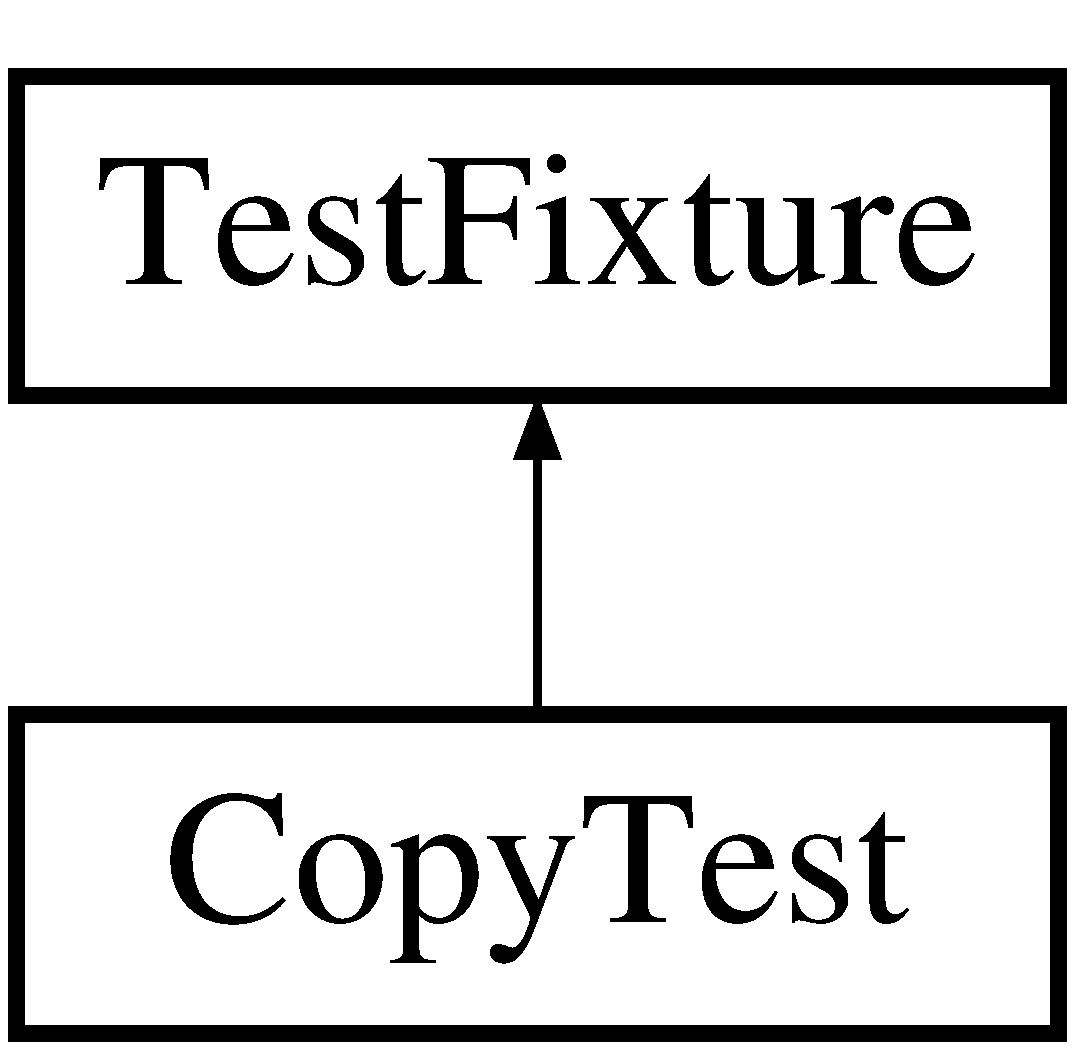
\includegraphics[height=2.000000cm]{class_copy_test}
\end{center}
\end{figure}
\subsection*{Metody publiczne}
\begin{DoxyCompactItemize}
\item 
void \hyperlink{class_copy_test_a753620e968ee6ac627e4e65ad139a54f}{copy\+\_\+constructor} ()
\item 
void \hyperlink{class_copy_test_aea0770d1ee3defbee564d72a7d3d9a44}{operator\+\_\+equal} ()
\item 
void \hyperlink{class_copy_test_a37811781b4c94cc5414b236290aae0d0}{operator\+\_\+equal\+\_\+non\+\_\+empty} ()
\end{DoxyCompactItemize}
\subsection*{Statyczne metody publiczne}
\begin{DoxyCompactItemize}
\item 
\mbox{\Hypertarget{class_copy_test_a9b9f546e882227c85841847274037bf4}\label{class_copy_test_a9b9f546e882227c85841847274037bf4}} 
static Test $\ast$ {\bfseries suite} ()
\end{DoxyCompactItemize}


\subsection{Dokumentacja funkcji składowych}
\mbox{\Hypertarget{class_copy_test_a753620e968ee6ac627e4e65ad139a54f}\label{class_copy_test_a753620e968ee6ac627e4e65ad139a54f}} 
\index{Copy\+Test@{Copy\+Test}!copy\+\_\+constructor@{copy\+\_\+constructor}}
\index{copy\+\_\+constructor@{copy\+\_\+constructor}!Copy\+Test@{Copy\+Test}}
\subsubsection{\texorpdfstring{copy\+\_\+constructor()}{copy\_constructor()}}
{\footnotesize\ttfamily void Copy\+Test\+::copy\+\_\+constructor (\begin{DoxyParamCaption}{ }\end{DoxyParamCaption})\hspace{0.3cm}{\ttfamily [inline]}}

Utworzono drzewo za pomocą konstruktora kopiującego \mbox{\Hypertarget{class_copy_test_aea0770d1ee3defbee564d72a7d3d9a44}\label{class_copy_test_aea0770d1ee3defbee564d72a7d3d9a44}} 
\index{Copy\+Test@{Copy\+Test}!operator\+\_\+equal@{operator\+\_\+equal}}
\index{operator\+\_\+equal@{operator\+\_\+equal}!Copy\+Test@{Copy\+Test}}
\subsubsection{\texorpdfstring{operator\+\_\+equal()}{operator\_equal()}}
{\footnotesize\ttfamily void Copy\+Test\+::operator\+\_\+equal (\begin{DoxyParamCaption}{ }\end{DoxyParamCaption})\hspace{0.3cm}{\ttfamily [inline]}}

Przypisano do pustego drzewa inne drzewo. \mbox{\Hypertarget{class_copy_test_a37811781b4c94cc5414b236290aae0d0}\label{class_copy_test_a37811781b4c94cc5414b236290aae0d0}} 
\index{Copy\+Test@{Copy\+Test}!operator\+\_\+equal\+\_\+non\+\_\+empty@{operator\+\_\+equal\+\_\+non\+\_\+empty}}
\index{operator\+\_\+equal\+\_\+non\+\_\+empty@{operator\+\_\+equal\+\_\+non\+\_\+empty}!Copy\+Test@{Copy\+Test}}
\subsubsection{\texorpdfstring{operator\+\_\+equal\+\_\+non\+\_\+empty()}{operator\_equal\_non\_empty()}}
{\footnotesize\ttfamily void Copy\+Test\+::operator\+\_\+equal\+\_\+non\+\_\+empty (\begin{DoxyParamCaption}{ }\end{DoxyParamCaption})\hspace{0.3cm}{\ttfamily [inline]}}

Przpisano do niepustego drzewa innego drzewo. 

Dokumentacja dla tej klasy została wygenerowana z pliku\+:\begin{DoxyCompactItemize}
\item 
test.\+cpp\end{DoxyCompactItemize}

\hypertarget{class_drzewo}{}\section{Drzewo$<$ T $>$ Class Template Reference}
\label{class_drzewo}\index{Drzewo$<$ T $>$@{Drzewo$<$ T $>$}}


{\ttfamily \#include $<$drzewo.\+hpp$>$}

\subsection*{Classes}
\begin{DoxyCompactItemize}
\item 
class \hyperlink{class_drzewo_1_1iterator}{iterator}
\end{DoxyCompactItemize}
\subsection*{Public Types}
\begin{DoxyCompactItemize}
\item 
\mbox{\Hypertarget{class_drzewo_a349719391d8470c24d68e8a4f0fecf3c}\label{class_drzewo_a349719391d8470c24d68e8a4f0fecf3c}} 
typedef T {\bfseries value\+\_\+type}
\item 
\mbox{\Hypertarget{class_drzewo_ad9689c01b3f07d1601e199799fcc1705}\label{class_drzewo_ad9689c01b3f07d1601e199799fcc1705}} 
typedef T \& {\bfseries reference}
\end{DoxyCompactItemize}
\subsection*{Public Member Functions}
\begin{DoxyCompactItemize}
\item 
\hyperlink{class_drzewo_a9b87f8101458fea6c866ffd01efa9ef6}{Drzewo} ()
\item 
\hyperlink{class_drzewo_a18f9e596cec9dd18eed19f2b613a7c44}{Drzewo} (const T \&root\+\_\+value)
\item 
\hyperlink{class_drzewo_a337d26f83b35b414b729a147e8995c3e}{Drzewo} (const \hyperlink{class_drzewo}{Drzewo} \&other\+\_\+tree)
\item 
\hyperlink{class_drzewo}{Drzewo} \& \hyperlink{class_drzewo_a409545162097a3cfa6072717c3fd710f}{operator=} (const \hyperlink{class_drzewo}{Drzewo} \&other\+\_\+tree)
\item 
\hyperlink{class_drzewo_acbc76af50077660d8a75eaa4e086eac1}{$\sim$\+Drzewo} ()
\item 
\hyperlink{class_drzewo_1_1iterator}{iterator} \hyperlink{class_drzewo_a3d00b2880e12a416ab749c84ff879a70}{insert} (const T \&value, \hyperlink{class_drzewo_1_1iterator}{iterator} parent, std\+::size\+\_\+t index)
\item 
void \hyperlink{class_drzewo_a338ae0e9b48ee6d513b9f99c81da3d4b}{erase} (const \hyperlink{class_drzewo_1_1iterator}{iterator} \&it)
\item 
\hyperlink{class_drzewo_1_1iterator}{iterator} \hyperlink{class_drzewo_ae45271ae9e1b1071d56c87df7eb37cad}{get\+Child} (const \hyperlink{class_drzewo_1_1iterator}{iterator} \&parent, std\+::size\+\_\+t index)
\item 
\hyperlink{class_drzewo_1_1iterator}{iterator} \hyperlink{class_drzewo_a2f6661025ebf9a3f6c2df1726a0d46ca}{begin} () const
\item 
\hyperlink{class_drzewo_1_1iterator}{iterator} \hyperlink{class_drzewo_aea36f65c42299dd029a38fbf9ed346fb}{end} () const
\item 
\hyperlink{class_drzewo_1_1iterator}{iterator} \hyperlink{class_drzewo_a86f9dd2d9c43b63476cedc0bd14ee878}{root} () const
\item 
bool \hyperlink{class_drzewo_abee09a10667c74ea82f4325addfac3df}{empty} ()
\item 
std\+::size\+\_\+t \hyperlink{class_drzewo_a778ee17b16674b9d0577d22f5d55fa04}{size} () const
\item 
int \hyperlink{class_drzewo_a0f5f70f7dfe35ffce3bb5ba3ac23657b}{get\+Number\+Of\+Children} (const \hyperlink{class_drzewo_1_1iterator}{iterator} \&parent)
\end{DoxyCompactItemize}


\subsection{Detailed Description}
\subsubsection*{template$<$typename T$>$\newline
class Drzewo$<$ T $>$}

Kontener reprezentujący strukturę danych -\/ \hyperlink{class_drzewo}{Drzewo}. Posiada korzeń, który jest jednocześnie węzłem/elementem w kontenerze. Istnieje możliwość utworzenia pustego drzewa. Dostęp do elementów kontenera jest udostępniony za pomocą pomocniczych obiektów klasy iterator. Obiekty 

\subsection{Constructor \& Destructor Documentation}
\mbox{\Hypertarget{class_drzewo_a9b87f8101458fea6c866ffd01efa9ef6}\label{class_drzewo_a9b87f8101458fea6c866ffd01efa9ef6}} 
\index{Drzewo@{Drzewo}!Drzewo@{Drzewo}}
\index{Drzewo@{Drzewo}!Drzewo@{Drzewo}}
\subsubsection{\texorpdfstring{Drzewo()}{Drzewo()}\hspace{0.1cm}{\footnotesize\ttfamily [1/3]}}
{\footnotesize\ttfamily template$<$typename T $>$ \\
\hyperlink{class_drzewo}{Drzewo}$<$ T $>$\+::\hyperlink{class_drzewo}{Drzewo} (\begin{DoxyParamCaption}{ }\end{DoxyParamCaption})}

Konstruktor domyślny. Inicjuje wkaźnik do korzenia na \textquotesingle{}nullptr\textquotesingle{}. Nowo utworzone drzewo posiada 0 węzłów. Zostanie utworzone puste drzewo. \mbox{\Hypertarget{class_drzewo_a18f9e596cec9dd18eed19f2b613a7c44}\label{class_drzewo_a18f9e596cec9dd18eed19f2b613a7c44}} 
\index{Drzewo@{Drzewo}!Drzewo@{Drzewo}}
\index{Drzewo@{Drzewo}!Drzewo@{Drzewo}}
\subsubsection{\texorpdfstring{Drzewo()}{Drzewo()}\hspace{0.1cm}{\footnotesize\ttfamily [2/3]}}
{\footnotesize\ttfamily template$<$typename T $>$ \\
\hyperlink{class_drzewo}{Drzewo}$<$ T $>$\+::\hyperlink{class_drzewo}{Drzewo} (\begin{DoxyParamCaption}\item[{const T \&}]{root\+\_\+value }\end{DoxyParamCaption})}

Konstruktor inicjujący korzeń drzewa wartością \textquotesingle{}root\+\_\+vale\textquotesingle{}. Zostanie utworzone drzewo z jednym węzłem.


\begin{DoxyParams}{Parameters}
{\em root\+\_\+value} & obiekt typu T. \\
\hline
\end{DoxyParams}
\mbox{\Hypertarget{class_drzewo_a337d26f83b35b414b729a147e8995c3e}\label{class_drzewo_a337d26f83b35b414b729a147e8995c3e}} 
\index{Drzewo@{Drzewo}!Drzewo@{Drzewo}}
\index{Drzewo@{Drzewo}!Drzewo@{Drzewo}}
\subsubsection{\texorpdfstring{Drzewo()}{Drzewo()}\hspace{0.1cm}{\footnotesize\ttfamily [3/3]}}
{\footnotesize\ttfamily template$<$typename T $>$ \\
\hyperlink{class_drzewo}{Drzewo}$<$ T $>$\+::\hyperlink{class_drzewo}{Drzewo} (\begin{DoxyParamCaption}\item[{const \hyperlink{class_drzewo}{Drzewo}$<$ T $>$ \&}]{other\+\_\+tree }\end{DoxyParamCaption})}

Konstruktor kopiujący, przyjmujący stałą referencję do innego drzewa. Wszystkie elementy drzewa kopiowanego zostają dodane do obecnie tworzonego drzewa, zachowując porządek, kolejność oraz hierarchię elementów.


\begin{DoxyParams}{Parameters}
{\em other\+\_\+tree} & obiekt klasy Drzewo$<$$>$. \\
\hline
\end{DoxyParams}
\mbox{\Hypertarget{class_drzewo_acbc76af50077660d8a75eaa4e086eac1}\label{class_drzewo_acbc76af50077660d8a75eaa4e086eac1}} 
\index{Drzewo@{Drzewo}!````~Drzewo@{$\sim$\+Drzewo}}
\index{````~Drzewo@{$\sim$\+Drzewo}!Drzewo@{Drzewo}}
\subsubsection{\texorpdfstring{$\sim$\+Drzewo()}{~Drzewo()}}
{\footnotesize\ttfamily template$<$typename T $>$ \\
\hyperlink{class_drzewo}{Drzewo}$<$ T $>$\+::$\sim$\hyperlink{class_drzewo}{Drzewo} (\begin{DoxyParamCaption}{ }\end{DoxyParamCaption})}

Destruktor, zwalnia pamięć, która była używana przez drzewo. Opróżnia wszystkie informacje zawarte w pojedynczych węzłach drzewa.


\begin{DoxyParams}{Parameters}
{\em (brak)} & \\
\hline
\end{DoxyParams}


\subsection{Member Function Documentation}
\mbox{\Hypertarget{class_drzewo_a2f6661025ebf9a3f6c2df1726a0d46ca}\label{class_drzewo_a2f6661025ebf9a3f6c2df1726a0d46ca}} 
\index{Drzewo@{Drzewo}!begin@{begin}}
\index{begin@{begin}!Drzewo@{Drzewo}}
\subsubsection{\texorpdfstring{begin()}{begin()}}
{\footnotesize\ttfamily template$<$typename T $>$ \\
\hyperlink{class_drzewo}{Drzewo}$<$ T $>$\+::\hyperlink{class_drzewo_1_1iterator}{iterator} \hyperlink{class_drzewo}{Drzewo}$<$ T $>$\+::begin (\begin{DoxyParamCaption}{ }\end{DoxyParamCaption}) const\hspace{0.3cm}{\ttfamily [inline]}}

Zwraca iterator pokazujący na pierwszy element w drzewie.


\begin{DoxyParams}{Parameters}
{\em (brak)} & \\
\hline
\end{DoxyParams}
\begin{DoxyReturn}{Returns}
iterator pokazujący na pierwszy element w drzewie. 
\end{DoxyReturn}
\mbox{\Hypertarget{class_drzewo_abee09a10667c74ea82f4325addfac3df}\label{class_drzewo_abee09a10667c74ea82f4325addfac3df}} 
\index{Drzewo@{Drzewo}!empty@{empty}}
\index{empty@{empty}!Drzewo@{Drzewo}}
\subsubsection{\texorpdfstring{empty()}{empty()}}
{\footnotesize\ttfamily template$<$typename T $>$ \\
bool \hyperlink{class_drzewo}{Drzewo}$<$ T $>$\+::empty (\begin{DoxyParamCaption}{ }\end{DoxyParamCaption})\hspace{0.3cm}{\ttfamily [inline]}}

Zwraca wartość \textquotesingle{}true\textquotesingle{} jeśli ilość węzłów w drzewie wynosi 0.


\begin{DoxyParams}{Parameters}
{\em (brak)} & \\
\hline
\end{DoxyParams}
\begin{DoxyReturn}{Returns}
true -\/ jeżeli liczba węzłów w drzewie równa się 0 false -\/ jeżeli liczba węzłów w drzwie jest większa od 0 
\end{DoxyReturn}
\mbox{\Hypertarget{class_drzewo_aea36f65c42299dd029a38fbf9ed346fb}\label{class_drzewo_aea36f65c42299dd029a38fbf9ed346fb}} 
\index{Drzewo@{Drzewo}!end@{end}}
\index{end@{end}!Drzewo@{Drzewo}}
\subsubsection{\texorpdfstring{end()}{end()}}
{\footnotesize\ttfamily template$<$typename T $>$ \\
\hyperlink{class_drzewo}{Drzewo}$<$ T $>$\+::\hyperlink{class_drzewo_1_1iterator}{iterator} \hyperlink{class_drzewo}{Drzewo}$<$ T $>$\+::end (\begin{DoxyParamCaption}{ }\end{DoxyParamCaption}) const\hspace{0.3cm}{\ttfamily [inline]}}

Zwraca iterator pokazujący na element za ostatnim elementem w drzewie.


\begin{DoxyParams}{Parameters}
{\em (brak)} & \\
\hline
\end{DoxyParams}
\begin{DoxyReturn}{Returns}
iterator 
\end{DoxyReturn}
\mbox{\Hypertarget{class_drzewo_a338ae0e9b48ee6d513b9f99c81da3d4b}\label{class_drzewo_a338ae0e9b48ee6d513b9f99c81da3d4b}} 
\index{Drzewo@{Drzewo}!erase@{erase}}
\index{erase@{erase}!Drzewo@{Drzewo}}
\subsubsection{\texorpdfstring{erase()}{erase()}}
{\footnotesize\ttfamily template$<$typename T $>$ \\
void \hyperlink{class_drzewo}{Drzewo}$<$ T $>$\+::erase (\begin{DoxyParamCaption}\item[{const \hyperlink{class_drzewo_1_1iterator}{iterator} \&}]{it }\end{DoxyParamCaption})}

Usuwa z drzewa element pokazywany przez iterator. W pierwszej kolejności zostaną usunięte wszystkie dzieci podanego węzła -\/ dealokacja pamięci. Jeśli dany węzeł posiada wiele poziomów dzieci, to zostaną najpierw usunięte wszystkie dzieci na najniższym poziomie drzewa, a następnie ich rodzice. Na końcu zostanie usunięty węzeł pokazywany przez iterator.


\begin{DoxyParams}{Parameters}
{\em it} & iterator pokazujący na węzeł przeznaczony do usunięcia. \\
\hline
\end{DoxyParams}
\mbox{\Hypertarget{class_drzewo_ae45271ae9e1b1071d56c87df7eb37cad}\label{class_drzewo_ae45271ae9e1b1071d56c87df7eb37cad}} 
\index{Drzewo@{Drzewo}!get\+Child@{get\+Child}}
\index{get\+Child@{get\+Child}!Drzewo@{Drzewo}}
\subsubsection{\texorpdfstring{get\+Child()}{getChild()}}
{\footnotesize\ttfamily template$<$typename T $>$ \\
\hyperlink{class_drzewo}{Drzewo}$<$ T $>$\+::\hyperlink{class_drzewo_1_1iterator}{iterator} \hyperlink{class_drzewo}{Drzewo}$<$ T $>$\+::get\+Child (\begin{DoxyParamCaption}\item[{const \hyperlink{class_drzewo_1_1iterator}{iterator} \&}]{parent,  }\item[{std\+::size\+\_\+t}]{index }\end{DoxyParamCaption})\hspace{0.3cm}{\ttfamily [inline]}}

Zwraca dziecko znajdujące się w liście dzieci węzła-\/rodzica wskazanego przez iterator, na miejscu o podanym indeksie.


\begin{DoxyParams}{Parameters}
{\em parent} & iterator na wezeł-\/rodzica \\
\hline
{\em index} & numer dziecka w liście dzieci rodzica \\
\hline
\end{DoxyParams}
\begin{DoxyReturn}{Returns}
iterator pokazujący na dziecko znajdujące się na danej pozycji 
\end{DoxyReturn}
\mbox{\Hypertarget{class_drzewo_a0f5f70f7dfe35ffce3bb5ba3ac23657b}\label{class_drzewo_a0f5f70f7dfe35ffce3bb5ba3ac23657b}} 
\index{Drzewo@{Drzewo}!get\+Number\+Of\+Children@{get\+Number\+Of\+Children}}
\index{get\+Number\+Of\+Children@{get\+Number\+Of\+Children}!Drzewo@{Drzewo}}
\subsubsection{\texorpdfstring{get\+Number\+Of\+Children()}{getNumberOfChildren()}}
{\footnotesize\ttfamily template$<$typename T $>$ \\
int \hyperlink{class_drzewo}{Drzewo}$<$ T $>$\+::get\+Number\+Of\+Children (\begin{DoxyParamCaption}\item[{const \hyperlink{class_drzewo_1_1iterator}{iterator} \&}]{parent }\end{DoxyParamCaption})\hspace{0.3cm}{\ttfamily [inline]}}

Zwraca liczbę \textquotesingle{}bezpośrednich\textquotesingle{} (znajdujących się bezpośrednio poziom pod danym węzłem) dzieci danego węzła, na który pokazuje iterator.


\begin{DoxyParams}{Parameters}
{\em parent} & iterator pokazujący na węzeł. \\
\hline
\end{DoxyParams}
\begin{DoxyReturn}{Returns}
liczba dzieci podanego rodzica. 
\end{DoxyReturn}
\mbox{\Hypertarget{class_drzewo_a3d00b2880e12a416ab749c84ff879a70}\label{class_drzewo_a3d00b2880e12a416ab749c84ff879a70}} 
\index{Drzewo@{Drzewo}!insert@{insert}}
\index{insert@{insert}!Drzewo@{Drzewo}}
\subsubsection{\texorpdfstring{insert()}{insert()}}
{\footnotesize\ttfamily template$<$typename T $>$ \\
\hyperlink{class_drzewo}{Drzewo}$<$ T $>$\+::\hyperlink{class_drzewo_1_1iterator}{iterator} \hyperlink{class_drzewo}{Drzewo}$<$ T $>$\+::insert (\begin{DoxyParamCaption}\item[{const T \&}]{value,  }\item[{\hyperlink{class_drzewo_1_1iterator}{iterator}}]{parent,  }\item[{std\+::size\+\_\+t}]{index }\end{DoxyParamCaption})}

Wstawia element o podanej wartości do drzewa, do listy dzieci rodzica, wskazywanego przez iterator, na określoną pozycję. W przypadku pustego drzewa oraz podania iteratora wskazującego na koniec kontenera oraz indexu równego \textquotesingle{}0\textquotesingle{} zostanie utworzony korzeń zawierający obiekt \textquotesingle{}value\textquotesingle{}. Zwrócony zostanie iterator pokazujący na korzeń drzewa.

W przypadku wywołania procedury insert z argumentami\+: iterator pokazujący na koniec oraz indexem równym 0, na niepustym drzewie zachowanie funkcji jest niezdefiniowane.

W pozostałych przypadkach element o wartości \textquotesingle{}value\textquotesingle{} zostanie wstawiony do listy dzieci węzła-\/rodzica pokazywanego przez iterator przed węzeł znajdujący się na miejscu nr \textquotesingle{}index\textquotesingle{}. Na koniec procedury zostanie zwiększona liczba elementów w drzewie.


\begin{DoxyParams}{Parameters}
{\em value} & obiekt typu T \\
\hline
{\em parent} & iterator pokazujący na węzeł-\/rodzic \\
\hline
{\em index} & numer pozycji na liście dzieci rodzica \\
\hline
\end{DoxyParams}
\begin{DoxyReturn}{Returns}
iterator pokazujący na nowo wstawione dziecko 
\end{DoxyReturn}
\mbox{\Hypertarget{class_drzewo_a409545162097a3cfa6072717c3fd710f}\label{class_drzewo_a409545162097a3cfa6072717c3fd710f}} 
\index{Drzewo@{Drzewo}!operator=@{operator=}}
\index{operator=@{operator=}!Drzewo@{Drzewo}}
\subsubsection{\texorpdfstring{operator=()}{operator=()}}
{\footnotesize\ttfamily template$<$typename T $>$ \\
\hyperlink{class_drzewo}{Drzewo}$<$ T $>$ \& \hyperlink{class_drzewo}{Drzewo}$<$ T $>$\+::operator= (\begin{DoxyParamCaption}\item[{const \hyperlink{class_drzewo}{Drzewo}$<$ T $>$ \&}]{other\+\_\+tree }\end{DoxyParamCaption})}

Operator przypisania drzewa. Przypisuje wszystkie elementy kopiowanego drzewa do obecnie tworzonego drzewa. Jeśli obecne drzewo nie jest puste, następuje wyczyszczenie wszystkich elementów drzewa, a następnie kopia. W przypadku wykonania operacji na pustych drzewach zostanie zwrócone puste drzewo.


\begin{DoxyParams}{Parameters}
{\em other\+\_\+tree} & obiekt klasy Drzewo$<$$>$. \\
\hline
\end{DoxyParams}
\mbox{\Hypertarget{class_drzewo_a86f9dd2d9c43b63476cedc0bd14ee878}\label{class_drzewo_a86f9dd2d9c43b63476cedc0bd14ee878}} 
\index{Drzewo@{Drzewo}!root@{root}}
\index{root@{root}!Drzewo@{Drzewo}}
\subsubsection{\texorpdfstring{root()}{root()}}
{\footnotesize\ttfamily template$<$typename T $>$ \\
\hyperlink{class_drzewo}{Drzewo}$<$ T $>$\+::\hyperlink{class_drzewo_1_1iterator}{iterator} \hyperlink{class_drzewo}{Drzewo}$<$ T $>$\+::root (\begin{DoxyParamCaption}{ }\end{DoxyParamCaption}) const\hspace{0.3cm}{\ttfamily [inline]}}

Zwraca iterator pokazujący na korzeń drzewa.


\begin{DoxyParams}{Parameters}
{\em (brak)} & \\
\hline
\end{DoxyParams}
\begin{DoxyReturn}{Returns}
iterator pokazujący na korzeń drzewa. 
\end{DoxyReturn}
\mbox{\Hypertarget{class_drzewo_a778ee17b16674b9d0577d22f5d55fa04}\label{class_drzewo_a778ee17b16674b9d0577d22f5d55fa04}} 
\index{Drzewo@{Drzewo}!size@{size}}
\index{size@{size}!Drzewo@{Drzewo}}
\subsubsection{\texorpdfstring{size()}{size()}}
{\footnotesize\ttfamily template$<$typename T $>$ \\
std\+::size\+\_\+t \hyperlink{class_drzewo}{Drzewo}$<$ T $>$\+::size (\begin{DoxyParamCaption}{ }\end{DoxyParamCaption}) const\hspace{0.3cm}{\ttfamily [inline]}}

Zwraca liczbę elementów występujących w drzewie.


\begin{DoxyParams}{Parameters}
{\em (brak)} & \\
\hline
\end{DoxyParams}
\begin{DoxyReturn}{Returns}
Liczba dzieci w drzewie. 
\end{DoxyReturn}


The documentation for this class was generated from the following file\+:\begin{DoxyCompactItemize}
\item 
drzewo.\+hpp\end{DoxyCompactItemize}

\hypertarget{class_empty_test}{}\section{Dokumentacja klasy Empty\+Test}
\label{class_empty_test}\index{Empty\+Test@{Empty\+Test}}
Diagram dziedziczenia dla Empty\+Test\begin{figure}[H]
\begin{center}
\leavevmode
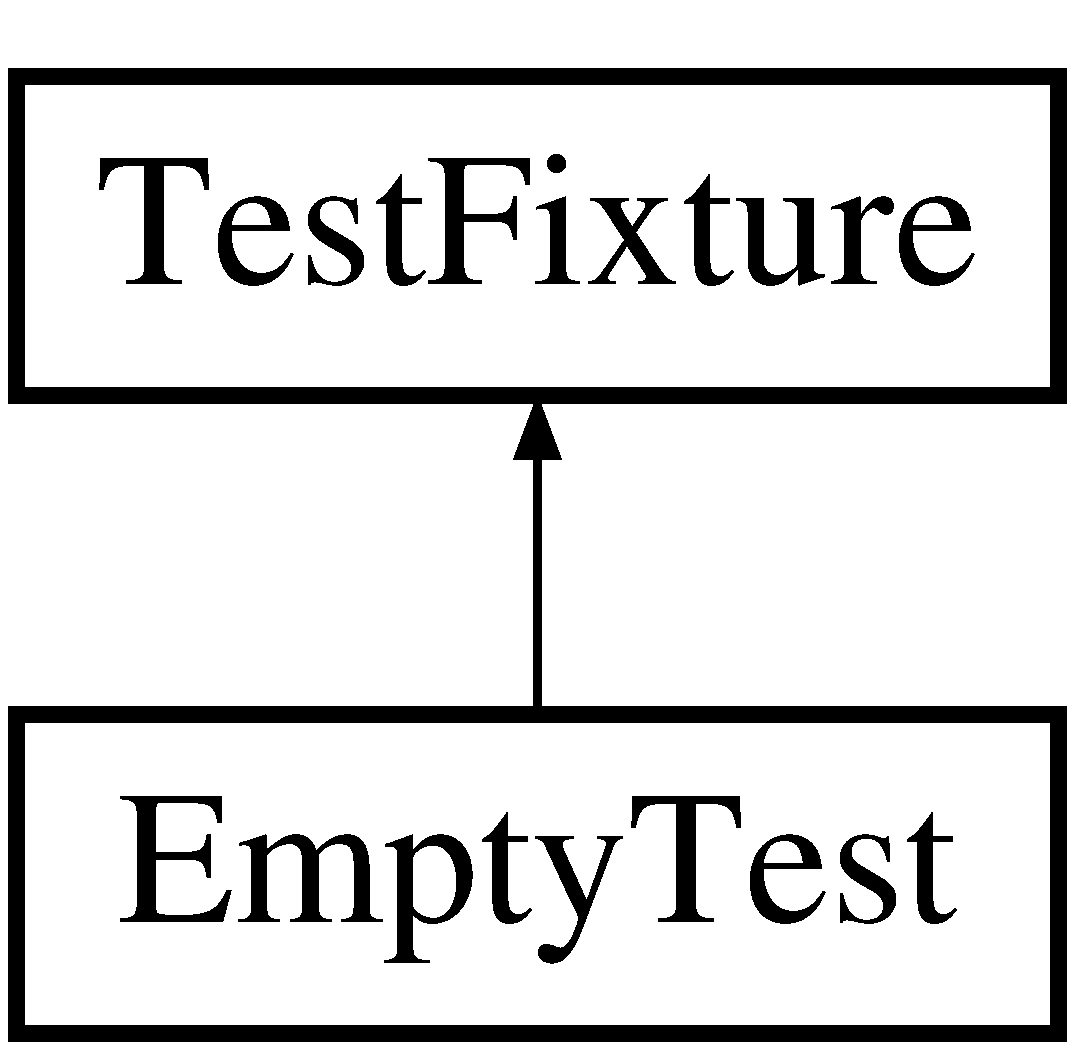
\includegraphics[height=2.000000cm]{class_empty_test}
\end{center}
\end{figure}
\subsection*{Metody publiczne}
\begin{DoxyCompactItemize}
\item 
void \hyperlink{class_empty_test_a27a72313c820dae24223b04c4f1cc376}{empty\+\_\+without\+\_\+root} ()
\item 
void \hyperlink{class_empty_test_abd96646c19026d62a5317285cbf5f49b}{empty\+\_\+with\+\_\+root} ()
\item 
void \hyperlink{class_empty_test_ad17133b184176d9d8b0511168d13ca6b}{empty\+\_\+without\+\_\+root\+\_\+insert} ()
\item 
void \hyperlink{class_empty_test_a5112f76f08ce5f0b52016ea8a8afff4b}{empty\+\_\+with\+\_\+root\+\_\+erase} ()
\item 
void \hyperlink{class_empty_test_a6a62d370484dd86a856514d168d176d4}{empty\+\_\+with\+\_\+root\+\_\+insert\+\_\+erase} ()
\item 
void \hyperlink{class_empty_test_a07de70993f853c66e95865432fc4ce7f}{empty\+\_\+with\+\_\+children\+\_\+erase\+\_\+root} ()
\item 
void \hyperlink{class_empty_test_a6373058c0b937d07bb07b8482f663315}{empty\+\_\+other\+\_\+tree} ()
\end{DoxyCompactItemize}
\subsection*{Statyczne metody publiczne}
\begin{DoxyCompactItemize}
\item 
\mbox{\Hypertarget{class_empty_test_a48e2fa8b65dab0443ba90e57289a58cf}\label{class_empty_test_a48e2fa8b65dab0443ba90e57289a58cf}} 
static Test $\ast$ {\bfseries suite} ()
\end{DoxyCompactItemize}


\subsection{Dokumentacja funkcji składowych}
\mbox{\Hypertarget{class_empty_test_a6373058c0b937d07bb07b8482f663315}\label{class_empty_test_a6373058c0b937d07bb07b8482f663315}} 
\index{Empty\+Test@{Empty\+Test}!empty\+\_\+other\+\_\+tree@{empty\+\_\+other\+\_\+tree}}
\index{empty\+\_\+other\+\_\+tree@{empty\+\_\+other\+\_\+tree}!Empty\+Test@{Empty\+Test}}
\subsubsection{\texorpdfstring{empty\+\_\+other\+\_\+tree()}{empty\_other\_tree()}}
{\footnotesize\ttfamily void Empty\+Test\+::empty\+\_\+other\+\_\+tree (\begin{DoxyParamCaption}{ }\end{DoxyParamCaption})\hspace{0.3cm}{\ttfamily [inline]}}

Do pustego drzewa przypisujemy inne puste drzewo \mbox{\Hypertarget{class_empty_test_a07de70993f853c66e95865432fc4ce7f}\label{class_empty_test_a07de70993f853c66e95865432fc4ce7f}} 
\index{Empty\+Test@{Empty\+Test}!empty\+\_\+with\+\_\+children\+\_\+erase\+\_\+root@{empty\+\_\+with\+\_\+children\+\_\+erase\+\_\+root}}
\index{empty\+\_\+with\+\_\+children\+\_\+erase\+\_\+root@{empty\+\_\+with\+\_\+children\+\_\+erase\+\_\+root}!Empty\+Test@{Empty\+Test}}
\subsubsection{\texorpdfstring{empty\+\_\+with\+\_\+children\+\_\+erase\+\_\+root()}{empty\_with\_children\_erase\_root()}}
{\footnotesize\ttfamily void Empty\+Test\+::empty\+\_\+with\+\_\+children\+\_\+erase\+\_\+root (\begin{DoxyParamCaption}{ }\end{DoxyParamCaption})\hspace{0.3cm}{\ttfamily [inline]}}

Dodano do drzewa dzieci, usunięto korzeń. \mbox{\Hypertarget{class_empty_test_abd96646c19026d62a5317285cbf5f49b}\label{class_empty_test_abd96646c19026d62a5317285cbf5f49b}} 
\index{Empty\+Test@{Empty\+Test}!empty\+\_\+with\+\_\+root@{empty\+\_\+with\+\_\+root}}
\index{empty\+\_\+with\+\_\+root@{empty\+\_\+with\+\_\+root}!Empty\+Test@{Empty\+Test}}
\subsubsection{\texorpdfstring{empty\+\_\+with\+\_\+root()}{empty\_with\_root()}}
{\footnotesize\ttfamily void Empty\+Test\+::empty\+\_\+with\+\_\+root (\begin{DoxyParamCaption}{ }\end{DoxyParamCaption})\hspace{0.3cm}{\ttfamily [inline]}}

Utworzono drzewo z wykorzystaniem konstruktora inicjującego \mbox{\Hypertarget{class_empty_test_a5112f76f08ce5f0b52016ea8a8afff4b}\label{class_empty_test_a5112f76f08ce5f0b52016ea8a8afff4b}} 
\index{Empty\+Test@{Empty\+Test}!empty\+\_\+with\+\_\+root\+\_\+erase@{empty\+\_\+with\+\_\+root\+\_\+erase}}
\index{empty\+\_\+with\+\_\+root\+\_\+erase@{empty\+\_\+with\+\_\+root\+\_\+erase}!Empty\+Test@{Empty\+Test}}
\subsubsection{\texorpdfstring{empty\+\_\+with\+\_\+root\+\_\+erase()}{empty\_with\_root\_erase()}}
{\footnotesize\ttfamily void Empty\+Test\+::empty\+\_\+with\+\_\+root\+\_\+erase (\begin{DoxyParamCaption}{ }\end{DoxyParamCaption})\hspace{0.3cm}{\ttfamily [inline]}}

Utworzono drzewo z korzeniem, następnie usunięto korzeń \mbox{\Hypertarget{class_empty_test_a6a62d370484dd86a856514d168d176d4}\label{class_empty_test_a6a62d370484dd86a856514d168d176d4}} 
\index{Empty\+Test@{Empty\+Test}!empty\+\_\+with\+\_\+root\+\_\+insert\+\_\+erase@{empty\+\_\+with\+\_\+root\+\_\+insert\+\_\+erase}}
\index{empty\+\_\+with\+\_\+root\+\_\+insert\+\_\+erase@{empty\+\_\+with\+\_\+root\+\_\+insert\+\_\+erase}!Empty\+Test@{Empty\+Test}}
\subsubsection{\texorpdfstring{empty\+\_\+with\+\_\+root\+\_\+insert\+\_\+erase()}{empty\_with\_root\_insert\_erase()}}
{\footnotesize\ttfamily void Empty\+Test\+::empty\+\_\+with\+\_\+root\+\_\+insert\+\_\+erase (\begin{DoxyParamCaption}{ }\end{DoxyParamCaption})\hspace{0.3cm}{\ttfamily [inline]}}

Utworzono drzewo bez korzenia, dodano korzeń, usunięto korzeń \mbox{\Hypertarget{class_empty_test_a27a72313c820dae24223b04c4f1cc376}\label{class_empty_test_a27a72313c820dae24223b04c4f1cc376}} 
\index{Empty\+Test@{Empty\+Test}!empty\+\_\+without\+\_\+root@{empty\+\_\+without\+\_\+root}}
\index{empty\+\_\+without\+\_\+root@{empty\+\_\+without\+\_\+root}!Empty\+Test@{Empty\+Test}}
\subsubsection{\texorpdfstring{empty\+\_\+without\+\_\+root()}{empty\_without\_root()}}
{\footnotesize\ttfamily void Empty\+Test\+::empty\+\_\+without\+\_\+root (\begin{DoxyParamCaption}{ }\end{DoxyParamCaption})\hspace{0.3cm}{\ttfamily [inline]}}

Utworzono drzewo z konstruktorem domyślnym \mbox{\Hypertarget{class_empty_test_ad17133b184176d9d8b0511168d13ca6b}\label{class_empty_test_ad17133b184176d9d8b0511168d13ca6b}} 
\index{Empty\+Test@{Empty\+Test}!empty\+\_\+without\+\_\+root\+\_\+insert@{empty\+\_\+without\+\_\+root\+\_\+insert}}
\index{empty\+\_\+without\+\_\+root\+\_\+insert@{empty\+\_\+without\+\_\+root\+\_\+insert}!Empty\+Test@{Empty\+Test}}
\subsubsection{\texorpdfstring{empty\+\_\+without\+\_\+root\+\_\+insert()}{empty\_without\_root\_insert()}}
{\footnotesize\ttfamily void Empty\+Test\+::empty\+\_\+without\+\_\+root\+\_\+insert (\begin{DoxyParamCaption}{ }\end{DoxyParamCaption})\hspace{0.3cm}{\ttfamily [inline]}}

Utworzono puste drzewo, a następnie dodano korzeń 

Dokumentacja dla tej klasy została wygenerowana z pliku\+:\begin{DoxyCompactItemize}
\item 
test.\+cpp\end{DoxyCompactItemize}

\hypertarget{class_erase_test}{}\section{Erase\+Test Class Reference}
\label{class_erase_test}\index{Erase\+Test@{Erase\+Test}}
Inheritance diagram for Erase\+Test\+:\begin{figure}[H]
\begin{center}
\leavevmode
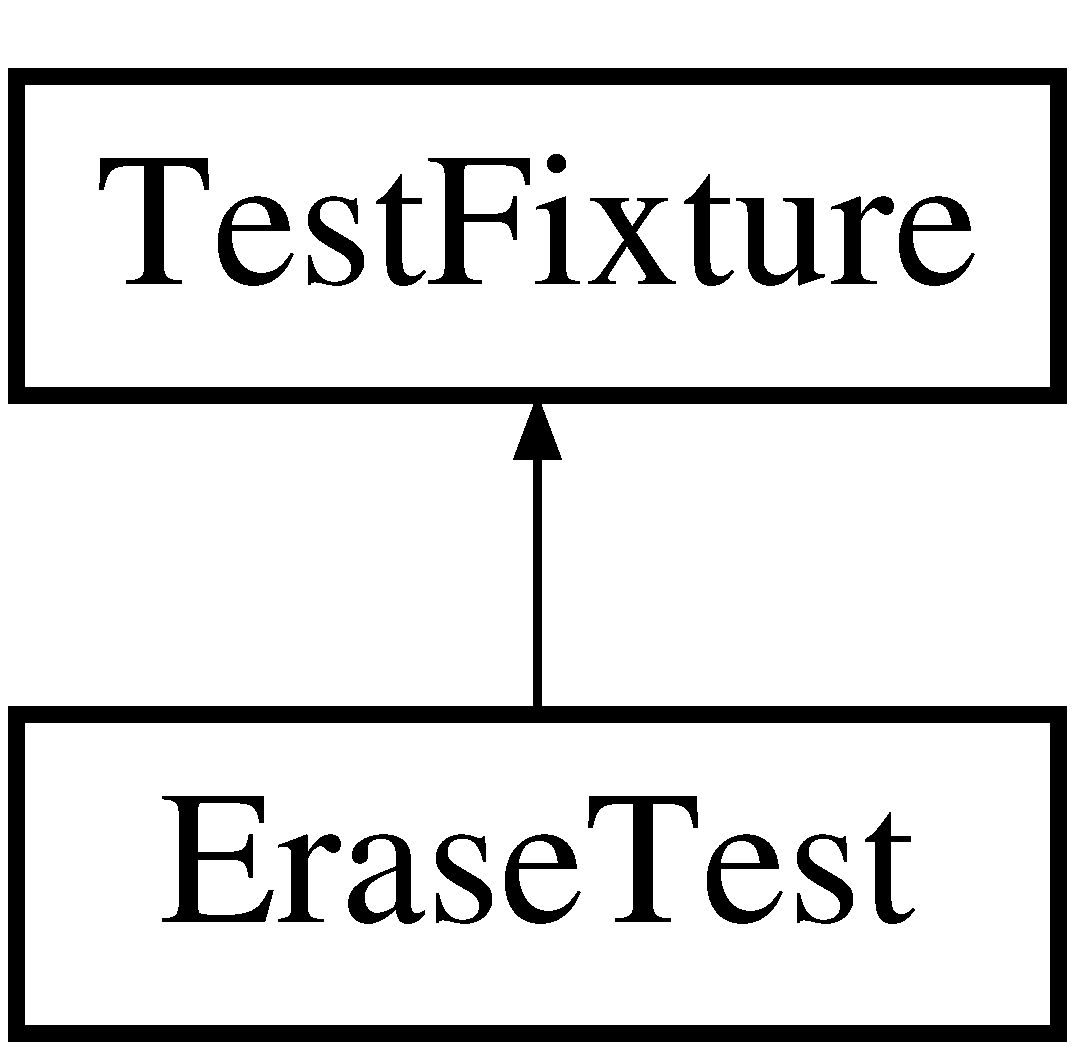
\includegraphics[height=2.000000cm]{class_erase_test}
\end{center}
\end{figure}
\subsection*{Public Member Functions}
\begin{DoxyCompactItemize}
\item 
void \hyperlink{class_erase_test_aa245715a2bbbcf0bd6abcca1a0992055}{erase\+\_\+root} ()
\item 
void \hyperlink{class_erase_test_ae6bc0aa4ecaa1f2966a0e4f971d229d1}{erase\+\_\+middle\+\_\+child} ()
\item 
void \hyperlink{class_erase_test_a0897542be38d32150b6c080449bf0b2d}{erase\+\_\+child\+\_\+shift} ()
\item 
void \hyperlink{class_erase_test_a3b1971101ff3dc813242f02a0cff68bf}{erase\+\_\+root\+\_\+value} ()
\item 
void \hyperlink{class_erase_test_a7c3b732833940974b289fd52f1190306}{erase\+\_\+many\+\_\+children} ()
\item 
void \hyperlink{class_erase_test_ac80cbc1c11f5ca0f218f0632b5b368b5}{delete\+\_\+tree\+\_\+many\+\_\+times} ()
\end{DoxyCompactItemize}
\subsection*{Static Public Member Functions}
\begin{DoxyCompactItemize}
\item 
\mbox{\Hypertarget{class_erase_test_ae12b35171f770e9f26decc0edc4c3206}\label{class_erase_test_ae12b35171f770e9f26decc0edc4c3206}} 
static Test $\ast$ {\bfseries suite} ()
\end{DoxyCompactItemize}


\subsection{Member Function Documentation}
\mbox{\Hypertarget{class_erase_test_ac80cbc1c11f5ca0f218f0632b5b368b5}\label{class_erase_test_ac80cbc1c11f5ca0f218f0632b5b368b5}} 
\index{Erase\+Test@{Erase\+Test}!delete\+\_\+tree\+\_\+many\+\_\+times@{delete\+\_\+tree\+\_\+many\+\_\+times}}
\index{delete\+\_\+tree\+\_\+many\+\_\+times@{delete\+\_\+tree\+\_\+many\+\_\+times}!Erase\+Test@{Erase\+Test}}
\subsubsection{\texorpdfstring{delete\+\_\+tree\+\_\+many\+\_\+times()}{delete\_tree\_many\_times()}}
{\footnotesize\ttfamily void Erase\+Test\+::delete\+\_\+tree\+\_\+many\+\_\+times (\begin{DoxyParamCaption}{ }\end{DoxyParamCaption})\hspace{0.3cm}{\ttfamily [inline]}}

Bardzo rozbudowane drzewo, usuwamy wiele razy i tworzymy wiele razy \mbox{\Hypertarget{class_erase_test_a0897542be38d32150b6c080449bf0b2d}\label{class_erase_test_a0897542be38d32150b6c080449bf0b2d}} 
\index{Erase\+Test@{Erase\+Test}!erase\+\_\+child\+\_\+shift@{erase\+\_\+child\+\_\+shift}}
\index{erase\+\_\+child\+\_\+shift@{erase\+\_\+child\+\_\+shift}!Erase\+Test@{Erase\+Test}}
\subsubsection{\texorpdfstring{erase\+\_\+child\+\_\+shift()}{erase\_child\_shift()}}
{\footnotesize\ttfamily void Erase\+Test\+::erase\+\_\+child\+\_\+shift (\begin{DoxyParamCaption}{ }\end{DoxyParamCaption})\hspace{0.3cm}{\ttfamily [inline]}}

Usunięto środkowe dziecko, sprawdzany porządek wśród dzieci. \mbox{\Hypertarget{class_erase_test_a7c3b732833940974b289fd52f1190306}\label{class_erase_test_a7c3b732833940974b289fd52f1190306}} 
\index{Erase\+Test@{Erase\+Test}!erase\+\_\+many\+\_\+children@{erase\+\_\+many\+\_\+children}}
\index{erase\+\_\+many\+\_\+children@{erase\+\_\+many\+\_\+children}!Erase\+Test@{Erase\+Test}}
\subsubsection{\texorpdfstring{erase\+\_\+many\+\_\+children()}{erase\_many\_children()}}
{\footnotesize\ttfamily void Erase\+Test\+::erase\+\_\+many\+\_\+children (\begin{DoxyParamCaption}{ }\end{DoxyParamCaption})\hspace{0.3cm}{\ttfamily [inline]}}

Usunięto wiele dzieci oraz danego rodzica. \mbox{\Hypertarget{class_erase_test_ae6bc0aa4ecaa1f2966a0e4f971d229d1}\label{class_erase_test_ae6bc0aa4ecaa1f2966a0e4f971d229d1}} 
\index{Erase\+Test@{Erase\+Test}!erase\+\_\+middle\+\_\+child@{erase\+\_\+middle\+\_\+child}}
\index{erase\+\_\+middle\+\_\+child@{erase\+\_\+middle\+\_\+child}!Erase\+Test@{Erase\+Test}}
\subsubsection{\texorpdfstring{erase\+\_\+middle\+\_\+child()}{erase\_middle\_child()}}
{\footnotesize\ttfamily void Erase\+Test\+::erase\+\_\+middle\+\_\+child (\begin{DoxyParamCaption}{ }\end{DoxyParamCaption})\hspace{0.3cm}{\ttfamily [inline]}}

Sprawdzana ilość dzieci \mbox{\Hypertarget{class_erase_test_aa245715a2bbbcf0bd6abcca1a0992055}\label{class_erase_test_aa245715a2bbbcf0bd6abcca1a0992055}} 
\index{Erase\+Test@{Erase\+Test}!erase\+\_\+root@{erase\+\_\+root}}
\index{erase\+\_\+root@{erase\+\_\+root}!Erase\+Test@{Erase\+Test}}
\subsubsection{\texorpdfstring{erase\+\_\+root()}{erase\_root()}}
{\footnotesize\ttfamily void Erase\+Test\+::erase\+\_\+root (\begin{DoxyParamCaption}{ }\end{DoxyParamCaption})\hspace{0.3cm}{\ttfamily [inline]}}

Usunięto korzeń. \mbox{\Hypertarget{class_erase_test_a3b1971101ff3dc813242f02a0cff68bf}\label{class_erase_test_a3b1971101ff3dc813242f02a0cff68bf}} 
\index{Erase\+Test@{Erase\+Test}!erase\+\_\+root\+\_\+value@{erase\+\_\+root\+\_\+value}}
\index{erase\+\_\+root\+\_\+value@{erase\+\_\+root\+\_\+value}!Erase\+Test@{Erase\+Test}}
\subsubsection{\texorpdfstring{erase\+\_\+root\+\_\+value()}{erase\_root\_value()}}
{\footnotesize\ttfamily void Erase\+Test\+::erase\+\_\+root\+\_\+value (\begin{DoxyParamCaption}{ }\end{DoxyParamCaption})\hspace{0.3cm}{\ttfamily [inline]}}

Sprawdzane poprawne przypisanie korzenia po usunięciu. 

The documentation for this class was generated from the following file\+:\begin{DoxyCompactItemize}
\item 
test.\+cpp\end{DoxyCompactItemize}

\hypertarget{class_get_child_test}{}\section{Dokumentacja klasy Get\+Child\+Test}
\label{class_get_child_test}\index{Get\+Child\+Test@{Get\+Child\+Test}}
Diagram dziedziczenia dla Get\+Child\+Test\begin{figure}[H]
\begin{center}
\leavevmode
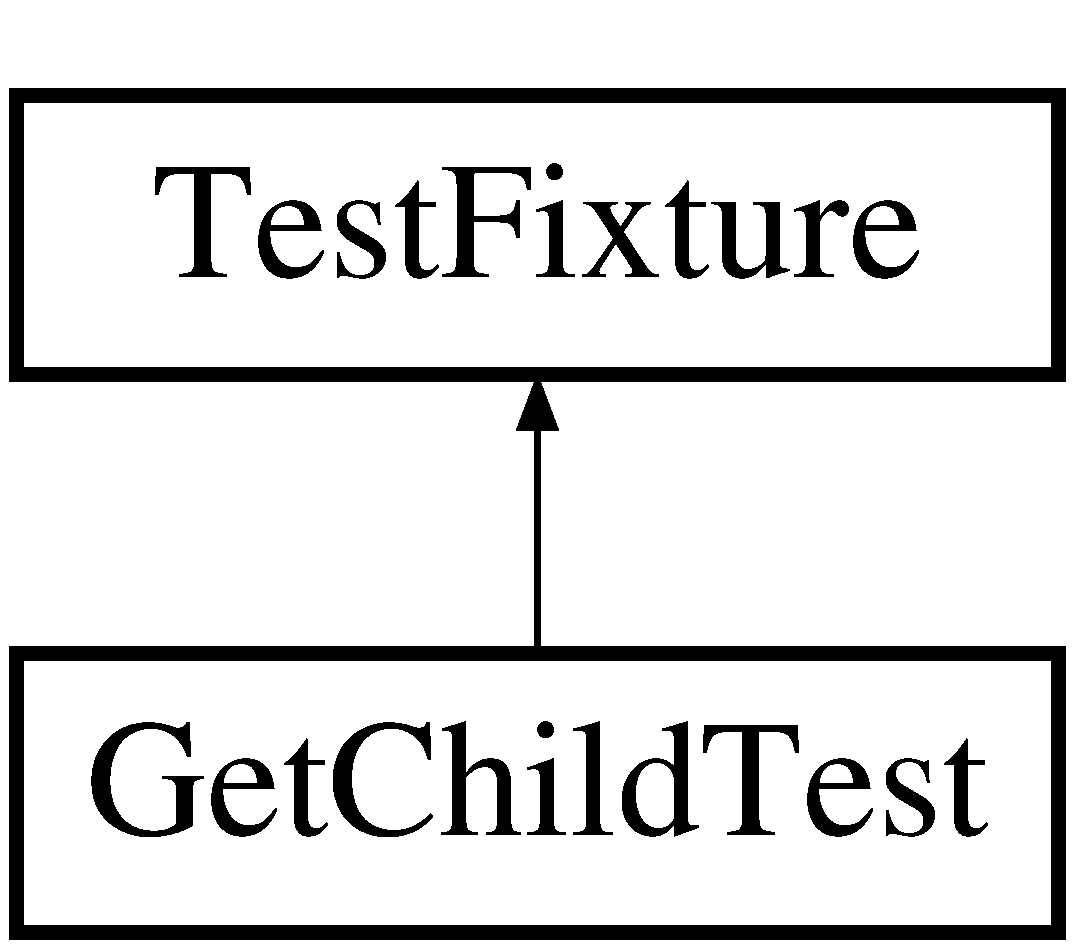
\includegraphics[height=2.000000cm]{class_get_child_test}
\end{center}
\end{figure}
\subsection*{Metody publiczne}
\begin{DoxyCompactItemize}
\item 
void \hyperlink{class_get_child_test_a1385e9059ba424b000d5e15ab28bd19b}{root\+\_\+children} ()
\item 
void \hyperlink{class_get_child_test_a3bbc21e060e29cdcc15708c2f3d7d8d1}{insert\+\_\+between} ()
\end{DoxyCompactItemize}
\subsection*{Statyczne metody publiczne}
\begin{DoxyCompactItemize}
\item 
\mbox{\Hypertarget{class_get_child_test_a4af2b9944cee3a7bf9f8a9ddc1729e47}\label{class_get_child_test_a4af2b9944cee3a7bf9f8a9ddc1729e47}} 
static Test $\ast$ {\bfseries suite} ()
\end{DoxyCompactItemize}


\subsection{Dokumentacja funkcji składowych}
\mbox{\Hypertarget{class_get_child_test_a3bbc21e060e29cdcc15708c2f3d7d8d1}\label{class_get_child_test_a3bbc21e060e29cdcc15708c2f3d7d8d1}} 
\index{Get\+Child\+Test@{Get\+Child\+Test}!insert\+\_\+between@{insert\+\_\+between}}
\index{insert\+\_\+between@{insert\+\_\+between}!Get\+Child\+Test@{Get\+Child\+Test}}
\subsubsection{\texorpdfstring{insert\+\_\+between()}{insert\_between()}}
{\footnotesize\ttfamily void Get\+Child\+Test\+::insert\+\_\+between (\begin{DoxyParamCaption}{ }\end{DoxyParamCaption})\hspace{0.3cm}{\ttfamily [inline]}}

wstawiamy pomiędzy dzieci i sprawdzamy czy poprawnie przesunęło \mbox{\Hypertarget{class_get_child_test_a1385e9059ba424b000d5e15ab28bd19b}\label{class_get_child_test_a1385e9059ba424b000d5e15ab28bd19b}} 
\index{Get\+Child\+Test@{Get\+Child\+Test}!root\+\_\+children@{root\+\_\+children}}
\index{root\+\_\+children@{root\+\_\+children}!Get\+Child\+Test@{Get\+Child\+Test}}
\subsubsection{\texorpdfstring{root\+\_\+children()}{root\_children()}}
{\footnotesize\ttfamily void Get\+Child\+Test\+::root\+\_\+children (\begin{DoxyParamCaption}{ }\end{DoxyParamCaption})\hspace{0.3cm}{\ttfamily [inline]}}

sprawdzamy dziecko korzenia 

Dokumentacja dla tej klasy została wygenerowana z pliku\+:\begin{DoxyCompactItemize}
\item 
test.\+cpp\end{DoxyCompactItemize}

\hypertarget{class_get_number_of_children_test}{}\section{Get\+Number\+Of\+Children\+Test Class Reference}
\label{class_get_number_of_children_test}\index{Get\+Number\+Of\+Children\+Test@{Get\+Number\+Of\+Children\+Test}}
Inheritance diagram for Get\+Number\+Of\+Children\+Test\+:\begin{figure}[H]
\begin{center}
\leavevmode
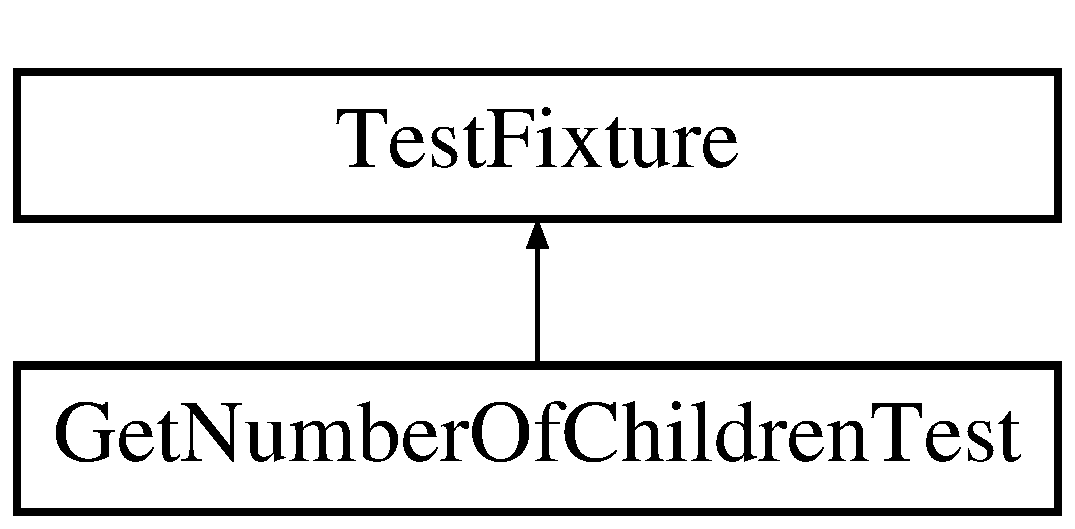
\includegraphics[height=2.000000cm]{class_get_number_of_children_test}
\end{center}
\end{figure}
\subsection*{Public Member Functions}
\begin{DoxyCompactItemize}
\item 
void \hyperlink{class_get_number_of_children_test_ab43b852fd1b487614fbb1799b54f723a}{root\+\_\+no\+\_\+children} ()
\item 
void \hyperlink{class_get_number_of_children_test_abf650bd374f47d9687109fb0022e5f21}{root\+\_\+children} ()
\item 
void \hyperlink{class_get_number_of_children_test_a0930a6f25c1f9d47424aab20a1733eb3}{node\+\_\+children\+\_\+insert} ()
\item 
void \hyperlink{class_get_number_of_children_test_ab19f7ecb2b671bc44fdfb2947deee52a}{node\+\_\+children\+\_\+erase} ()
\end{DoxyCompactItemize}
\subsection*{Static Public Member Functions}
\begin{DoxyCompactItemize}
\item 
\mbox{\Hypertarget{class_get_number_of_children_test_a348017e90bc30a00737ea03bfb44820d}\label{class_get_number_of_children_test_a348017e90bc30a00737ea03bfb44820d}} 
static Test $\ast$ {\bfseries suite} ()
\end{DoxyCompactItemize}


\subsection{Member Function Documentation}
\mbox{\Hypertarget{class_get_number_of_children_test_ab19f7ecb2b671bc44fdfb2947deee52a}\label{class_get_number_of_children_test_ab19f7ecb2b671bc44fdfb2947deee52a}} 
\index{Get\+Number\+Of\+Children\+Test@{Get\+Number\+Of\+Children\+Test}!node\+\_\+children\+\_\+erase@{node\+\_\+children\+\_\+erase}}
\index{node\+\_\+children\+\_\+erase@{node\+\_\+children\+\_\+erase}!Get\+Number\+Of\+Children\+Test@{Get\+Number\+Of\+Children\+Test}}
\subsubsection{\texorpdfstring{node\+\_\+children\+\_\+erase()}{node\_children\_erase()}}
{\footnotesize\ttfamily void Get\+Number\+Of\+Children\+Test\+::node\+\_\+children\+\_\+erase (\begin{DoxyParamCaption}{ }\end{DoxyParamCaption})\hspace{0.3cm}{\ttfamily [inline]}}

Dodano do korzenia dzieci, a następnie usunięto dziecko. \mbox{\Hypertarget{class_get_number_of_children_test_a0930a6f25c1f9d47424aab20a1733eb3}\label{class_get_number_of_children_test_a0930a6f25c1f9d47424aab20a1733eb3}} 
\index{Get\+Number\+Of\+Children\+Test@{Get\+Number\+Of\+Children\+Test}!node\+\_\+children\+\_\+insert@{node\+\_\+children\+\_\+insert}}
\index{node\+\_\+children\+\_\+insert@{node\+\_\+children\+\_\+insert}!Get\+Number\+Of\+Children\+Test@{Get\+Number\+Of\+Children\+Test}}
\subsubsection{\texorpdfstring{node\+\_\+children\+\_\+insert()}{node\_children\_insert()}}
{\footnotesize\ttfamily void Get\+Number\+Of\+Children\+Test\+::node\+\_\+children\+\_\+insert (\begin{DoxyParamCaption}{ }\end{DoxyParamCaption})\hspace{0.3cm}{\ttfamily [inline]}}

Dodano do korzenia dzieci, a nastepnie jeszcze jedno dziecko. \mbox{\Hypertarget{class_get_number_of_children_test_abf650bd374f47d9687109fb0022e5f21}\label{class_get_number_of_children_test_abf650bd374f47d9687109fb0022e5f21}} 
\index{Get\+Number\+Of\+Children\+Test@{Get\+Number\+Of\+Children\+Test}!root\+\_\+children@{root\+\_\+children}}
\index{root\+\_\+children@{root\+\_\+children}!Get\+Number\+Of\+Children\+Test@{Get\+Number\+Of\+Children\+Test}}
\subsubsection{\texorpdfstring{root\+\_\+children()}{root\_children()}}
{\footnotesize\ttfamily void Get\+Number\+Of\+Children\+Test\+::root\+\_\+children (\begin{DoxyParamCaption}{ }\end{DoxyParamCaption})\hspace{0.3cm}{\ttfamily [inline]}}

Utworzono drzewo i dodano do korzenia wiele dzieci \mbox{\Hypertarget{class_get_number_of_children_test_ab43b852fd1b487614fbb1799b54f723a}\label{class_get_number_of_children_test_ab43b852fd1b487614fbb1799b54f723a}} 
\index{Get\+Number\+Of\+Children\+Test@{Get\+Number\+Of\+Children\+Test}!root\+\_\+no\+\_\+children@{root\+\_\+no\+\_\+children}}
\index{root\+\_\+no\+\_\+children@{root\+\_\+no\+\_\+children}!Get\+Number\+Of\+Children\+Test@{Get\+Number\+Of\+Children\+Test}}
\subsubsection{\texorpdfstring{root\+\_\+no\+\_\+children()}{root\_no\_children()}}
{\footnotesize\ttfamily void Get\+Number\+Of\+Children\+Test\+::root\+\_\+no\+\_\+children (\begin{DoxyParamCaption}{ }\end{DoxyParamCaption})\hspace{0.3cm}{\ttfamily [inline]}}

Utworzono drzewo z korzeniem, bez dzieci. 

The documentation for this class was generated from the following file\+:\begin{DoxyCompactItemize}
\item 
test.\+cpp\end{DoxyCompactItemize}

\hypertarget{class_insert_test}{}\section{Insert\+Test Class Reference}
\label{class_insert_test}\index{Insert\+Test@{Insert\+Test}}
Inheritance diagram for Insert\+Test\+:\begin{figure}[H]
\begin{center}
\leavevmode
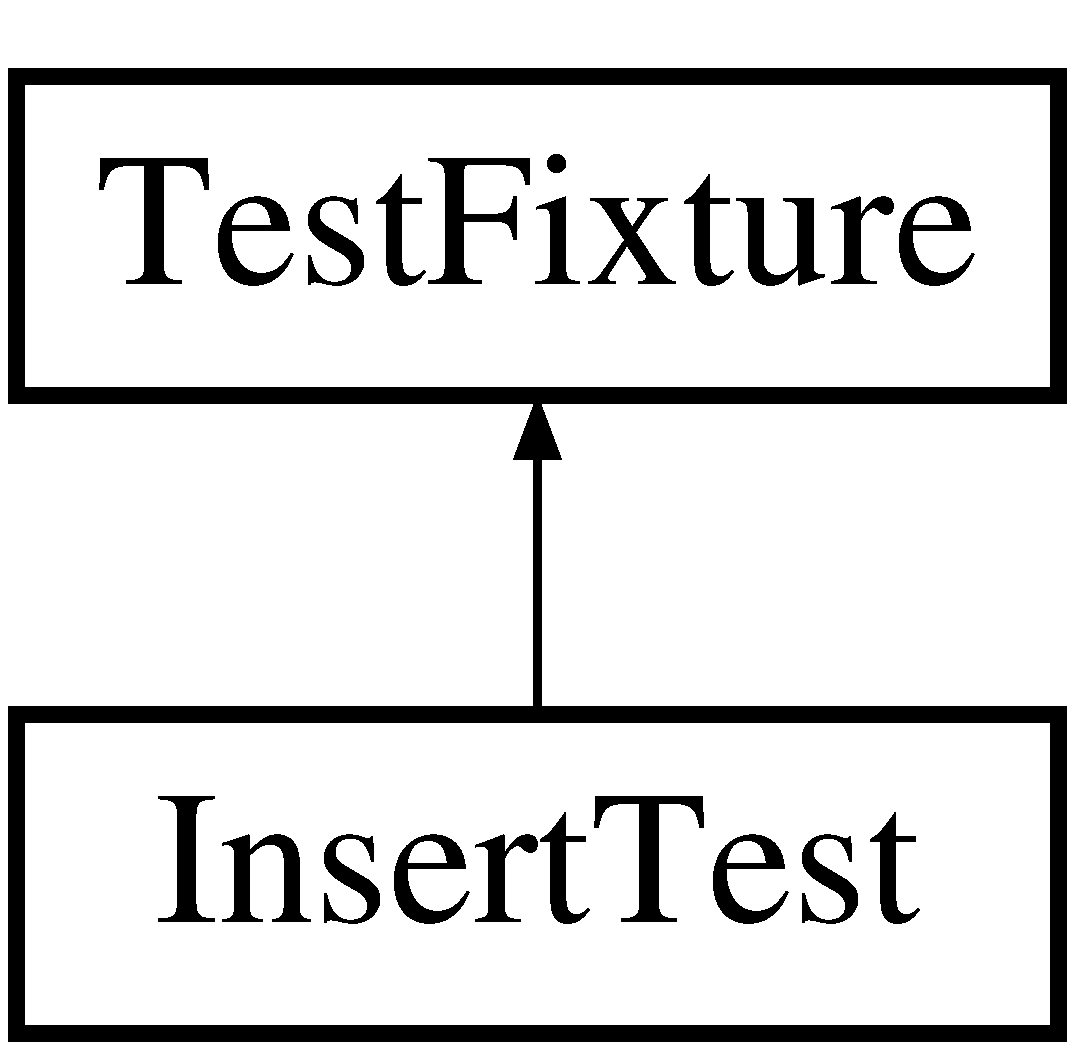
\includegraphics[height=2.000000cm]{class_insert_test}
\end{center}
\end{figure}
\subsection*{Public Member Functions}
\begin{DoxyCompactItemize}
\item 
void \hyperlink{class_insert_test_a08b1a1c6b86e528795c49c20e019d701}{insert\+\_\+root} ()
\item 
void \hyperlink{class_insert_test_a0bab461bf75465f1f23a21a962266389}{insert\+\_\+root\+\_\+child} ()
\item 
void \hyperlink{class_insert_test_aed04f1b62d643e9d6bfa713930a1805b}{insert\+\_\+front} ()
\end{DoxyCompactItemize}
\subsection*{Static Public Member Functions}
\begin{DoxyCompactItemize}
\item 
\mbox{\Hypertarget{class_insert_test_aebbf65f804a3b4af0545dc32211925a5}\label{class_insert_test_aebbf65f804a3b4af0545dc32211925a5}} 
static Test $\ast$ {\bfseries suite} ()
\end{DoxyCompactItemize}


\subsection{Member Function Documentation}
\mbox{\Hypertarget{class_insert_test_aed04f1b62d643e9d6bfa713930a1805b}\label{class_insert_test_aed04f1b62d643e9d6bfa713930a1805b}} 
\index{Insert\+Test@{Insert\+Test}!insert\+\_\+front@{insert\+\_\+front}}
\index{insert\+\_\+front@{insert\+\_\+front}!Insert\+Test@{Insert\+Test}}
\subsubsection{\texorpdfstring{insert\+\_\+front()}{insert\_front()}}
{\footnotesize\ttfamily void Insert\+Test\+::insert\+\_\+front (\begin{DoxyParamCaption}{ }\end{DoxyParamCaption})\hspace{0.3cm}{\ttfamily [inline]}}

Wstawiano zawsze jako pierwsze dziecko \mbox{\Hypertarget{class_insert_test_a08b1a1c6b86e528795c49c20e019d701}\label{class_insert_test_a08b1a1c6b86e528795c49c20e019d701}} 
\index{Insert\+Test@{Insert\+Test}!insert\+\_\+root@{insert\+\_\+root}}
\index{insert\+\_\+root@{insert\+\_\+root}!Insert\+Test@{Insert\+Test}}
\subsubsection{\texorpdfstring{insert\+\_\+root()}{insert\_root()}}
{\footnotesize\ttfamily void Insert\+Test\+::insert\+\_\+root (\begin{DoxyParamCaption}{ }\end{DoxyParamCaption})\hspace{0.3cm}{\ttfamily [inline]}}

Wstawion korzeń, sprawdzono rozmiar drzewa oraz iterator pokazujący na korzeń. \mbox{\Hypertarget{class_insert_test_a0bab461bf75465f1f23a21a962266389}\label{class_insert_test_a0bab461bf75465f1f23a21a962266389}} 
\index{Insert\+Test@{Insert\+Test}!insert\+\_\+root\+\_\+child@{insert\+\_\+root\+\_\+child}}
\index{insert\+\_\+root\+\_\+child@{insert\+\_\+root\+\_\+child}!Insert\+Test@{Insert\+Test}}
\subsubsection{\texorpdfstring{insert\+\_\+root\+\_\+child()}{insert\_root\_child()}}
{\footnotesize\ttfamily void Insert\+Test\+::insert\+\_\+root\+\_\+child (\begin{DoxyParamCaption}{ }\end{DoxyParamCaption})\hspace{0.3cm}{\ttfamily [inline]}}

Wstawiono dzieci do korzenia, porównano iteratory i liczby dzieci. 

The documentation for this class was generated from the following file\+:\begin{DoxyCompactItemize}
\item 
test.\+cpp\end{DoxyCompactItemize}

\hypertarget{class_drzewo_1_1iterator}{}\section{Drzewo$<$ T $>$\+:\+:iterator Class Reference}
\label{class_drzewo_1_1iterator}\index{Drzewo$<$ T $>$\+::iterator@{Drzewo$<$ T $>$\+::iterator}}
\subsection*{Public Types}
\begin{DoxyCompactItemize}
\item 
\mbox{\Hypertarget{class_drzewo_1_1iterator_a7ba4387023d41aafa83791b42fc5b5ee}\label{class_drzewo_1_1iterator_a7ba4387023d41aafa83791b42fc5b5ee}} 
typedef T {\bfseries value\+\_\+type}
\end{DoxyCompactItemize}
\subsection*{Public Member Functions}
\begin{DoxyCompactItemize}
\item 
\hyperlink{class_drzewo_1_1iterator_a279751514e51594342daa7a7ed501a38}{iterator} ()
\item 
\hyperlink{class_drzewo_1_1iterator_a627d8a55a11ad8be75493634c6fe07b2}{iterator} (const \hyperlink{class_drzewo_1_1iterator}{iterator} \&\hyperlink{class_drzewo_1_1iterator}{iterator})
\item 
T \& \hyperlink{class_drzewo_1_1iterator_ab2ee76d0390832e9bed32a829f08f328}{operator$\ast$} ()
\item 
\hyperlink{class_drzewo_1_1iterator}{iterator} \& \hyperlink{class_drzewo_1_1iterator_a8b67f4409ee4532a89e745744ba6f8b3}{operator++} ()
\item 
T $\ast$ \hyperlink{class_drzewo_1_1iterator_ac982660e25eb9720b5c81b6ccff0559e}{operator-\/$>$} ()
\item 
bool \hyperlink{class_drzewo_1_1iterator_a7bc726d05d85b2d7b2cd68f180237331}{operator!=} (const \hyperlink{class_drzewo_1_1iterator}{iterator} \&it)
\item 
bool \hyperlink{class_drzewo_1_1iterator_a552c4e6d4bb62519595329bc5cf32d98}{operator==} (const \hyperlink{class_drzewo_1_1iterator}{iterator} \&it)
\end{DoxyCompactItemize}
\subsection*{Friends}
\begin{DoxyCompactItemize}
\item 
\mbox{\Hypertarget{class_drzewo_1_1iterator_a1c4e4c3515fb1b999118d69c354d7efd}\label{class_drzewo_1_1iterator_a1c4e4c3515fb1b999118d69c354d7efd}} 
class {\bfseries Drzewo}
\end{DoxyCompactItemize}


\subsection{Constructor \& Destructor Documentation}
\mbox{\Hypertarget{class_drzewo_1_1iterator_a279751514e51594342daa7a7ed501a38}\label{class_drzewo_1_1iterator_a279751514e51594342daa7a7ed501a38}} 
\index{Drzewo\+::iterator@{Drzewo\+::iterator}!iterator@{iterator}}
\index{iterator@{iterator}!Drzewo\+::iterator@{Drzewo\+::iterator}}
\subsubsection{\texorpdfstring{iterator()}{iterator()}\hspace{0.1cm}{\footnotesize\ttfamily [1/2]}}
{\footnotesize\ttfamily template$<$typename T $>$ \\
\hyperlink{class_drzewo}{Drzewo}$<$ T $>$\+::iterator\+::iterator (\begin{DoxyParamCaption}{ }\end{DoxyParamCaption})\hspace{0.3cm}{\ttfamily [inline]}}

T Konstruktor domyślny ustawiający wskaźnik do węzła na \textquotesingle{}nullptr\textquotesingle{}.


\begin{DoxyParams}{Parameters}
{\em (brak)} & \\
\hline
\end{DoxyParams}
\mbox{\Hypertarget{class_drzewo_1_1iterator_a627d8a55a11ad8be75493634c6fe07b2}\label{class_drzewo_1_1iterator_a627d8a55a11ad8be75493634c6fe07b2}} 
\index{Drzewo\+::iterator@{Drzewo\+::iterator}!iterator@{iterator}}
\index{iterator@{iterator}!Drzewo\+::iterator@{Drzewo\+::iterator}}
\subsubsection{\texorpdfstring{iterator()}{iterator()}\hspace{0.1cm}{\footnotesize\ttfamily [2/2]}}
{\footnotesize\ttfamily template$<$typename T $>$ \\
\hyperlink{class_drzewo}{Drzewo}$<$ T $>$\+::iterator\+::iterator (\begin{DoxyParamCaption}\item[{const \hyperlink{class_drzewo_1_1iterator}{iterator} \&}]{iterator }\end{DoxyParamCaption})\hspace{0.3cm}{\ttfamily [inline]}}

Konstruktor kopiujący ustawiający wartość wskaźnika na wskaźnik pokazywany przez iterator.


\begin{DoxyParams}{Parameters}
{\em iterator} & iterator, którego wskaźnik zostanie skopiowany. \\
\hline
\end{DoxyParams}


\subsection{Member Function Documentation}
\mbox{\Hypertarget{class_drzewo_1_1iterator_a7bc726d05d85b2d7b2cd68f180237331}\label{class_drzewo_1_1iterator_a7bc726d05d85b2d7b2cd68f180237331}} 
\index{Drzewo\+::iterator@{Drzewo\+::iterator}!operator"!=@{operator"!=}}
\index{operator"!=@{operator"!=}!Drzewo\+::iterator@{Drzewo\+::iterator}}
\subsubsection{\texorpdfstring{operator"!=()}{operator!=()}}
{\footnotesize\ttfamily template$<$typename T $>$ \\
bool \hyperlink{class_drzewo}{Drzewo}$<$ T $>$\+::iterator\+::operator!= (\begin{DoxyParamCaption}\item[{const \hyperlink{class_drzewo_1_1iterator}{iterator} \&}]{it }\end{DoxyParamCaption})\hspace{0.3cm}{\ttfamily [inline]}}

Zwraca \textquotesingle{}true\textquotesingle{} jeśli iterator pokazuje na inny węzeł niż iterator przesyłany do funkcji.

\begin{DoxyReturn}{Returns}
true -\/ gdy obiekty na które pokazują iteratory są różne, flase -\/ gdy obiekty na które pokazują iteratory są równe 
\end{DoxyReturn}
\mbox{\Hypertarget{class_drzewo_1_1iterator_ab2ee76d0390832e9bed32a829f08f328}\label{class_drzewo_1_1iterator_ab2ee76d0390832e9bed32a829f08f328}} 
\index{Drzewo\+::iterator@{Drzewo\+::iterator}!operator$\ast$@{operator$\ast$}}
\index{operator$\ast$@{operator$\ast$}!Drzewo\+::iterator@{Drzewo\+::iterator}}
\subsubsection{\texorpdfstring{operator$\ast$()}{operator*()}}
{\footnotesize\ttfamily template$<$typename T $>$ \\
T \& \hyperlink{class_drzewo}{Drzewo}$<$ T $>$\+::iterator\+::operator$\ast$ (\begin{DoxyParamCaption}{ }\end{DoxyParamCaption})\hspace{0.3cm}{\ttfamily [inline]}}

Zwraca referencję do obiektu typu przechowywanego w pojedynczym węźle, wskazywanym przez iterator.


\begin{DoxyParams}{Parameters}
{\em (brak)} & \\
\hline
\end{DoxyParams}
\begin{DoxyReturn}{Returns}
referencja do obiektu typu T 
\end{DoxyReturn}
\mbox{\Hypertarget{class_drzewo_1_1iterator_a8b67f4409ee4532a89e745744ba6f8b3}\label{class_drzewo_1_1iterator_a8b67f4409ee4532a89e745744ba6f8b3}} 
\index{Drzewo\+::iterator@{Drzewo\+::iterator}!operator++@{operator++}}
\index{operator++@{operator++}!Drzewo\+::iterator@{Drzewo\+::iterator}}
\subsubsection{\texorpdfstring{operator++()}{operator++()}}
{\footnotesize\ttfamily template$<$typename T $>$ \\
\hyperlink{class_drzewo}{Drzewo}$<$ T $>$\+::\hyperlink{class_drzewo_1_1iterator}{iterator} \& \hyperlink{class_drzewo}{Drzewo}$<$ T $>$\+::iterator\+::operator++ (\begin{DoxyParamCaption}{ }\end{DoxyParamCaption})}


\begin{DoxyParams}{Parameters}
{\em (brak)} & \\
\hline
\end{DoxyParams}
\begin{DoxyReturn}{Returns}
Wskaźnik do samego siebie. 
\end{DoxyReturn}
\mbox{\Hypertarget{class_drzewo_1_1iterator_ac982660e25eb9720b5c81b6ccff0559e}\label{class_drzewo_1_1iterator_ac982660e25eb9720b5c81b6ccff0559e}} 
\index{Drzewo\+::iterator@{Drzewo\+::iterator}!operator-\/$>$@{operator-\/$>$}}
\index{operator-\/$>$@{operator-\/$>$}!Drzewo\+::iterator@{Drzewo\+::iterator}}
\subsubsection{\texorpdfstring{operator-\/$>$()}{operator->()}}
{\footnotesize\ttfamily template$<$typename T $>$ \\
T $\ast$ \hyperlink{class_drzewo}{Drzewo}$<$ T $>$\+::iterator\+::operator-\/$>$ (\begin{DoxyParamCaption}{ }\end{DoxyParamCaption})\hspace{0.3cm}{\ttfamily [inline]}}


\begin{DoxyParams}{Parameters}
{\em (brak)} & \\
\hline
\end{DoxyParams}
\mbox{\Hypertarget{class_drzewo_1_1iterator_a552c4e6d4bb62519595329bc5cf32d98}\label{class_drzewo_1_1iterator_a552c4e6d4bb62519595329bc5cf32d98}} 
\index{Drzewo\+::iterator@{Drzewo\+::iterator}!operator==@{operator==}}
\index{operator==@{operator==}!Drzewo\+::iterator@{Drzewo\+::iterator}}
\subsubsection{\texorpdfstring{operator==()}{operator==()}}
{\footnotesize\ttfamily template$<$typename T $>$ \\
bool \hyperlink{class_drzewo}{Drzewo}$<$ T $>$\+::iterator\+::operator== (\begin{DoxyParamCaption}\item[{const \hyperlink{class_drzewo_1_1iterator}{iterator} \&}]{it }\end{DoxyParamCaption})\hspace{0.3cm}{\ttfamily [inline]}}

Zwraca \textquotesingle{}true\textquotesingle{} jeśli iterator pokazuje na ten sam węzeł niż iterator przesyłany do funkcji.

\begin{DoxyReturn}{Returns}
true -\/ gdy obiekty na które pokazują iteratory są równe, flase -\/ gdy obiekty na które pokazują iteratory są różne 
\end{DoxyReturn}


The documentation for this class was generated from the following file\+:\begin{DoxyCompactItemize}
\item 
drzewo.\+hpp\end{DoxyCompactItemize}

\hypertarget{class_iterator_test}{}\section{Iterator\+Test Class Reference}
\label{class_iterator_test}\index{Iterator\+Test@{Iterator\+Test}}
Inheritance diagram for Iterator\+Test\+:\begin{figure}[H]
\begin{center}
\leavevmode
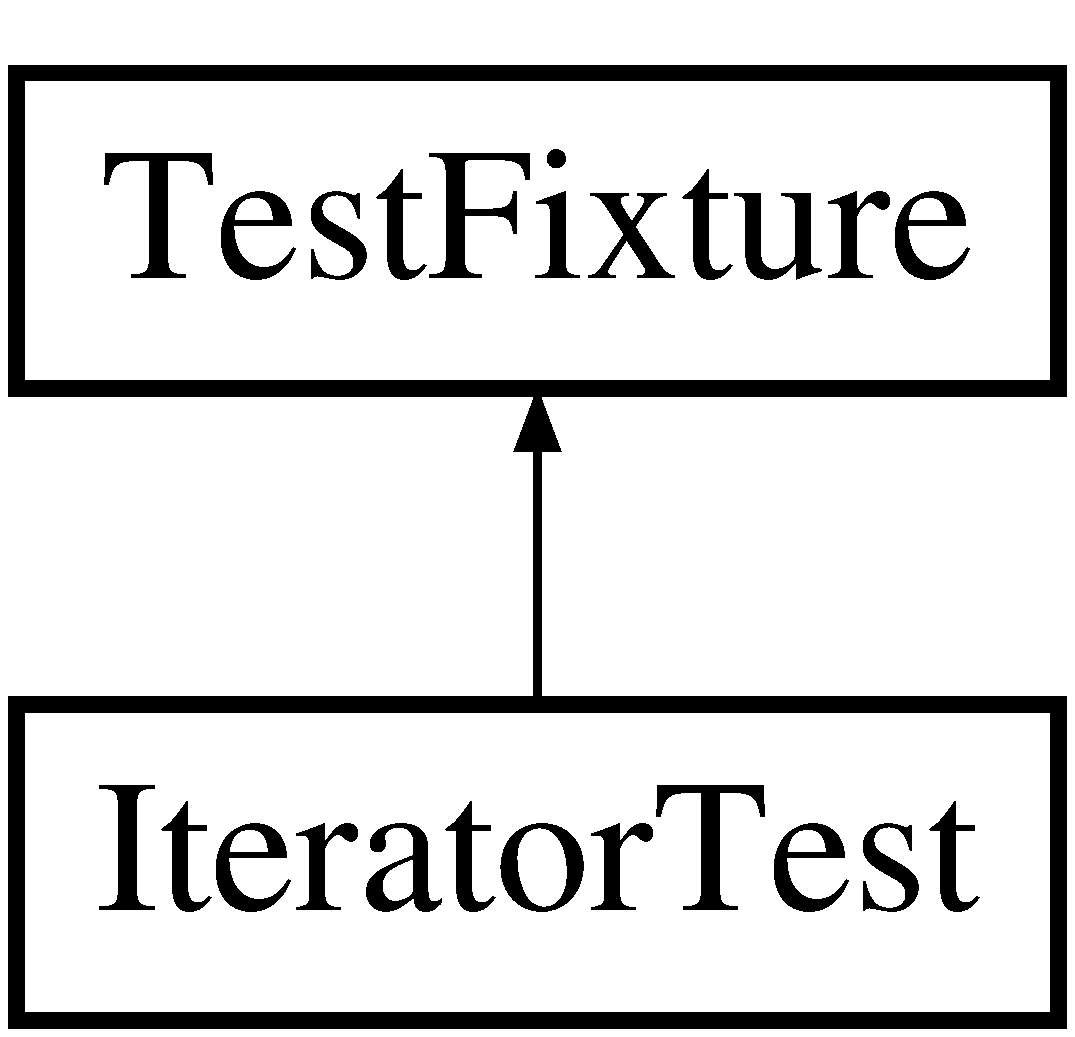
\includegraphics[height=2.000000cm]{class_iterator_test}
\end{center}
\end{figure}
\subsection*{Public Member Functions}
\begin{DoxyCompactItemize}
\item 
void \hyperlink{class_iterator_test_a9a97bde928f26d4482c1f422dff08b1e}{root\+\_\+test} ()
\item 
void \hyperlink{class_iterator_test_a4defa697edd8ac31231e2f437f5b01e5}{root\+\_\+erase} ()
\item 
void \hyperlink{class_iterator_test_a12ba95e8b8465d2378afd5db43efc6e5}{insert\+\_\+get\+\_\+child} ()
\item 
void \hyperlink{class_iterator_test_a7b80412e084b4a4502daddba5102e3c5}{operator\+\_\+asterisk} ()
\item 
void \hyperlink{class_iterator_test_a826f30ef86193414b8ceb03e76592b37}{empty\+\_\+tree} ()
\item 
void \hyperlink{class_iterator_test_acd1cdaec5c6d5a2b183bbb8dbd979c2a}{operator\+\_\+inequal} ()
\item 
void \hyperlink{class_iterator_test_a4bd66d05af2e1fc6c3d7850ccc7ac783}{operator\+\_\+equal} ()
\end{DoxyCompactItemize}
\subsection*{Static Public Member Functions}
\begin{DoxyCompactItemize}
\item 
\mbox{\Hypertarget{class_iterator_test_a5251aa78e108a94e3b969a784a74d5e6}\label{class_iterator_test_a5251aa78e108a94e3b969a784a74d5e6}} 
static Test $\ast$ {\bfseries suite} ()
\end{DoxyCompactItemize}


\subsection{Member Function Documentation}
\mbox{\Hypertarget{class_iterator_test_a826f30ef86193414b8ceb03e76592b37}\label{class_iterator_test_a826f30ef86193414b8ceb03e76592b37}} 
\index{Iterator\+Test@{Iterator\+Test}!empty\+\_\+tree@{empty\+\_\+tree}}
\index{empty\+\_\+tree@{empty\+\_\+tree}!Iterator\+Test@{Iterator\+Test}}
\subsubsection{\texorpdfstring{empty\+\_\+tree()}{empty\_tree()}}
{\footnotesize\ttfamily void Iterator\+Test\+::empty\+\_\+tree (\begin{DoxyParamCaption}{ }\end{DoxyParamCaption})\hspace{0.3cm}{\ttfamily [inline]}}

Sprawdzono, iterator na korzeń pokazuje na koniec w przypadku utworzenia pustego drzewa. \mbox{\Hypertarget{class_iterator_test_a12ba95e8b8465d2378afd5db43efc6e5}\label{class_iterator_test_a12ba95e8b8465d2378afd5db43efc6e5}} 
\index{Iterator\+Test@{Iterator\+Test}!insert\+\_\+get\+\_\+child@{insert\+\_\+get\+\_\+child}}
\index{insert\+\_\+get\+\_\+child@{insert\+\_\+get\+\_\+child}!Iterator\+Test@{Iterator\+Test}}
\subsubsection{\texorpdfstring{insert\+\_\+get\+\_\+child()}{insert\_get\_child()}}
{\footnotesize\ttfamily void Iterator\+Test\+::insert\+\_\+get\+\_\+child (\begin{DoxyParamCaption}{ }\end{DoxyParamCaption})\hspace{0.3cm}{\ttfamily [inline]}}

Sprawdzono czy iterator zwrócony przez insert i get\+Child pokazuje na ten sam element. \mbox{\Hypertarget{class_iterator_test_a7b80412e084b4a4502daddba5102e3c5}\label{class_iterator_test_a7b80412e084b4a4502daddba5102e3c5}} 
\index{Iterator\+Test@{Iterator\+Test}!operator\+\_\+asterisk@{operator\+\_\+asterisk}}
\index{operator\+\_\+asterisk@{operator\+\_\+asterisk}!Iterator\+Test@{Iterator\+Test}}
\subsubsection{\texorpdfstring{operator\+\_\+asterisk()}{operator\_asterisk()}}
{\footnotesize\ttfamily void Iterator\+Test\+::operator\+\_\+asterisk (\begin{DoxyParamCaption}{ }\end{DoxyParamCaption})\hspace{0.3cm}{\ttfamily [inline]}}

Sprawdzono poprawność operatora$\ast$ zwracającego wartość obiektu T przechowywanego w węźle. \mbox{\Hypertarget{class_iterator_test_a4bd66d05af2e1fc6c3d7850ccc7ac783}\label{class_iterator_test_a4bd66d05af2e1fc6c3d7850ccc7ac783}} 
\index{Iterator\+Test@{Iterator\+Test}!operator\+\_\+equal@{operator\+\_\+equal}}
\index{operator\+\_\+equal@{operator\+\_\+equal}!Iterator\+Test@{Iterator\+Test}}
\subsubsection{\texorpdfstring{operator\+\_\+equal()}{operator\_equal()}}
{\footnotesize\ttfamily void Iterator\+Test\+::operator\+\_\+equal (\begin{DoxyParamCaption}{ }\end{DoxyParamCaption})\hspace{0.3cm}{\ttfamily [inline]}}

Sprawdzanie poprawności działania oepratora == \mbox{\Hypertarget{class_iterator_test_acd1cdaec5c6d5a2b183bbb8dbd979c2a}\label{class_iterator_test_acd1cdaec5c6d5a2b183bbb8dbd979c2a}} 
\index{Iterator\+Test@{Iterator\+Test}!operator\+\_\+inequal@{operator\+\_\+inequal}}
\index{operator\+\_\+inequal@{operator\+\_\+inequal}!Iterator\+Test@{Iterator\+Test}}
\subsubsection{\texorpdfstring{operator\+\_\+inequal()}{operator\_inequal()}}
{\footnotesize\ttfamily void Iterator\+Test\+::operator\+\_\+inequal (\begin{DoxyParamCaption}{ }\end{DoxyParamCaption})\hspace{0.3cm}{\ttfamily [inline]}}

Sprawdzenie poprawności działania operatora != \mbox{\Hypertarget{class_iterator_test_a4defa697edd8ac31231e2f437f5b01e5}\label{class_iterator_test_a4defa697edd8ac31231e2f437f5b01e5}} 
\index{Iterator\+Test@{Iterator\+Test}!root\+\_\+erase@{root\+\_\+erase}}
\index{root\+\_\+erase@{root\+\_\+erase}!Iterator\+Test@{Iterator\+Test}}
\subsubsection{\texorpdfstring{root\+\_\+erase()}{root\_erase()}}
{\footnotesize\ttfamily void Iterator\+Test\+::root\+\_\+erase (\begin{DoxyParamCaption}{ }\end{DoxyParamCaption})\hspace{0.3cm}{\ttfamily [inline]}}

Usunięto korzeń, iterator powinien pokazuwać na koniec drzewa. \mbox{\Hypertarget{class_iterator_test_a9a97bde928f26d4482c1f422dff08b1e}\label{class_iterator_test_a9a97bde928f26d4482c1f422dff08b1e}} 
\index{Iterator\+Test@{Iterator\+Test}!root\+\_\+test@{root\+\_\+test}}
\index{root\+\_\+test@{root\+\_\+test}!Iterator\+Test@{Iterator\+Test}}
\subsubsection{\texorpdfstring{root\+\_\+test()}{root\_test()}}
{\footnotesize\ttfamily void Iterator\+Test\+::root\+\_\+test (\begin{DoxyParamCaption}{ }\end{DoxyParamCaption})\hspace{0.3cm}{\ttfamily [inline]}}

Sprawdzono czy iterator po wstawieniu korzenia pokazuje na korzeń drzewa. 

The documentation for this class was generated from the following file\+:\begin{DoxyCompactItemize}
\item 
test.\+cpp\end{DoxyCompactItemize}

\hypertarget{class_size_test}{}\section{Size\+Test Class Reference}
\label{class_size_test}\index{Size\+Test@{Size\+Test}}
Inheritance diagram for Size\+Test\+:\begin{figure}[H]
\begin{center}
\leavevmode
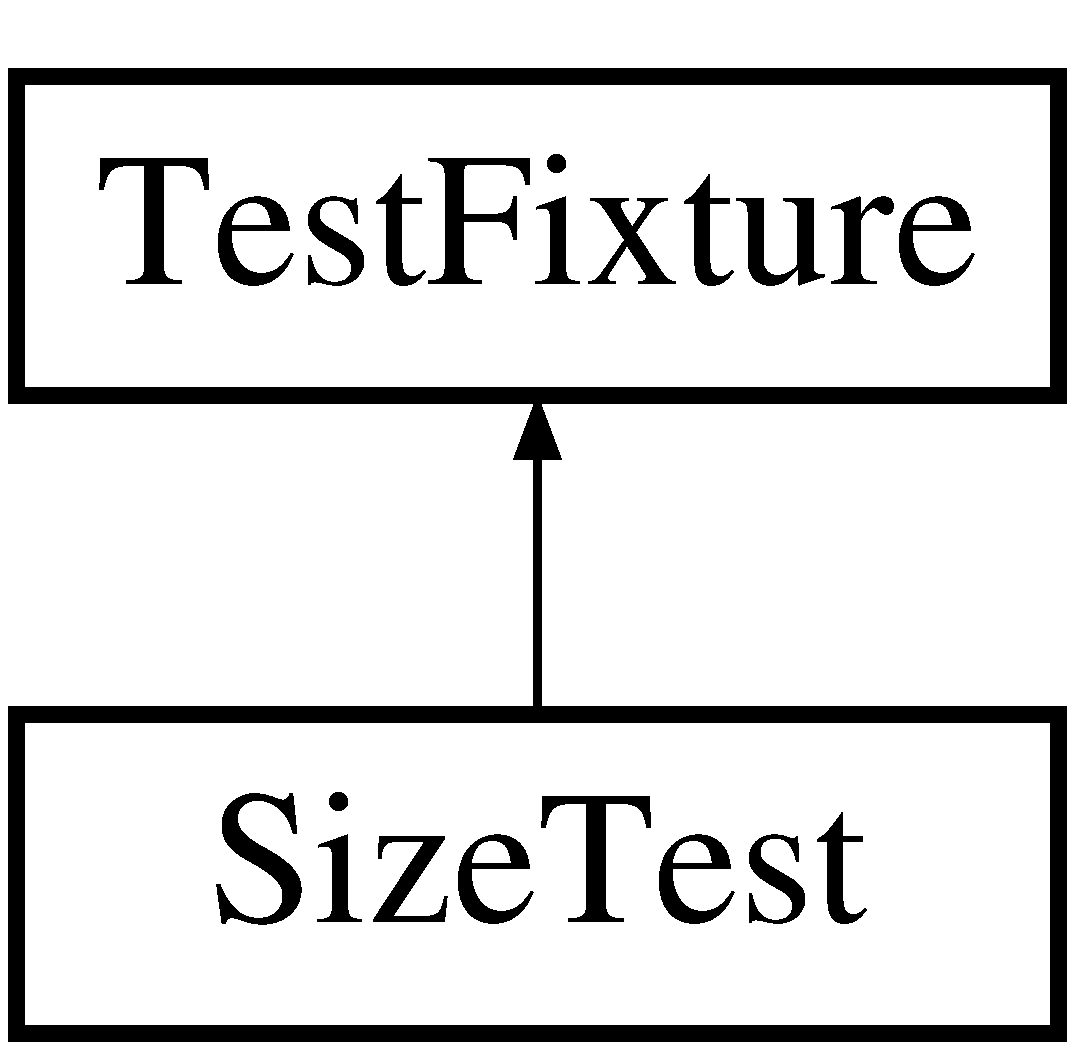
\includegraphics[height=2.000000cm]{class_size_test}
\end{center}
\end{figure}
\subsection*{Public Member Functions}
\begin{DoxyCompactItemize}
\item 
void \hyperlink{class_size_test_a85261b7c20794c5d64335ca31cdf37cf}{one\+\_\+element\+\_\+constructor} ()
\item 
void \hyperlink{class_size_test_a0aca43b07dd7f2dc7abb018193c7957a}{one\+\_\+element\+\_\+insert} ()
\item 
void \hyperlink{class_size_test_aaed7bed9e378c1d8f57b841b20f25caa}{zero\+\_\+elements} ()
\item 
void \hyperlink{class_size_test_a8746c855c3846914d88c34c061197682}{more\+\_\+elements} ()
\item 
void \hyperlink{class_size_test_a02868a105b57f585aaa7d435c3208d61}{more\+\_\+elements\+\_\+erase\+\_\+leaf} ()
\item 
void \hyperlink{class_size_test_addf81e5e704a50add6060c1810eabba9}{more\+\_\+elements\+\_\+erase\+\_\+parent} ()
\end{DoxyCompactItemize}
\subsection*{Static Public Member Functions}
\begin{DoxyCompactItemize}
\item 
\mbox{\Hypertarget{class_size_test_ad83c4e302657fd74119fbcc78f31e47f}\label{class_size_test_ad83c4e302657fd74119fbcc78f31e47f}} 
static Test $\ast$ {\bfseries suite} ()
\end{DoxyCompactItemize}


\subsection{Member Function Documentation}
\mbox{\Hypertarget{class_size_test_a8746c855c3846914d88c34c061197682}\label{class_size_test_a8746c855c3846914d88c34c061197682}} 
\index{Size\+Test@{Size\+Test}!more\+\_\+elements@{more\+\_\+elements}}
\index{more\+\_\+elements@{more\+\_\+elements}!Size\+Test@{Size\+Test}}
\subsubsection{\texorpdfstring{more\+\_\+elements()}{more\_elements()}}
{\footnotesize\ttfamily void Size\+Test\+::more\+\_\+elements (\begin{DoxyParamCaption}{ }\end{DoxyParamCaption})\hspace{0.3cm}{\ttfamily [inline]}}

Dodano więcej elementów \mbox{\Hypertarget{class_size_test_a02868a105b57f585aaa7d435c3208d61}\label{class_size_test_a02868a105b57f585aaa7d435c3208d61}} 
\index{Size\+Test@{Size\+Test}!more\+\_\+elements\+\_\+erase\+\_\+leaf@{more\+\_\+elements\+\_\+erase\+\_\+leaf}}
\index{more\+\_\+elements\+\_\+erase\+\_\+leaf@{more\+\_\+elements\+\_\+erase\+\_\+leaf}!Size\+Test@{Size\+Test}}
\subsubsection{\texorpdfstring{more\+\_\+elements\+\_\+erase\+\_\+leaf()}{more\_elements\_erase\_leaf()}}
{\footnotesize\ttfamily void Size\+Test\+::more\+\_\+elements\+\_\+erase\+\_\+leaf (\begin{DoxyParamCaption}{ }\end{DoxyParamCaption})\hspace{0.3cm}{\ttfamily [inline]}}

Dodano więcej elementów a potem usunięto liść \mbox{\Hypertarget{class_size_test_addf81e5e704a50add6060c1810eabba9}\label{class_size_test_addf81e5e704a50add6060c1810eabba9}} 
\index{Size\+Test@{Size\+Test}!more\+\_\+elements\+\_\+erase\+\_\+parent@{more\+\_\+elements\+\_\+erase\+\_\+parent}}
\index{more\+\_\+elements\+\_\+erase\+\_\+parent@{more\+\_\+elements\+\_\+erase\+\_\+parent}!Size\+Test@{Size\+Test}}
\subsubsection{\texorpdfstring{more\+\_\+elements\+\_\+erase\+\_\+parent()}{more\_elements\_erase\_parent()}}
{\footnotesize\ttfamily void Size\+Test\+::more\+\_\+elements\+\_\+erase\+\_\+parent (\begin{DoxyParamCaption}{ }\end{DoxyParamCaption})\hspace{0.3cm}{\ttfamily [inline]}}

usunięto rodzica, który miał dwoje dzieci \mbox{\Hypertarget{class_size_test_a85261b7c20794c5d64335ca31cdf37cf}\label{class_size_test_a85261b7c20794c5d64335ca31cdf37cf}} 
\index{Size\+Test@{Size\+Test}!one\+\_\+element\+\_\+constructor@{one\+\_\+element\+\_\+constructor}}
\index{one\+\_\+element\+\_\+constructor@{one\+\_\+element\+\_\+constructor}!Size\+Test@{Size\+Test}}
\subsubsection{\texorpdfstring{one\+\_\+element\+\_\+constructor()}{one\_element\_constructor()}}
{\footnotesize\ttfamily void Size\+Test\+::one\+\_\+element\+\_\+constructor (\begin{DoxyParamCaption}{ }\end{DoxyParamCaption})\hspace{0.3cm}{\ttfamily [inline]}}

Wywołano konstruktor inicjujący \mbox{\Hypertarget{class_size_test_a0aca43b07dd7f2dc7abb018193c7957a}\label{class_size_test_a0aca43b07dd7f2dc7abb018193c7957a}} 
\index{Size\+Test@{Size\+Test}!one\+\_\+element\+\_\+insert@{one\+\_\+element\+\_\+insert}}
\index{one\+\_\+element\+\_\+insert@{one\+\_\+element\+\_\+insert}!Size\+Test@{Size\+Test}}
\subsubsection{\texorpdfstring{one\+\_\+element\+\_\+insert()}{one\_element\_insert()}}
{\footnotesize\ttfamily void Size\+Test\+::one\+\_\+element\+\_\+insert (\begin{DoxyParamCaption}{ }\end{DoxyParamCaption})\hspace{0.3cm}{\ttfamily [inline]}}

wstawiono element do pustego drzewa \mbox{\Hypertarget{class_size_test_aaed7bed9e378c1d8f57b841b20f25caa}\label{class_size_test_aaed7bed9e378c1d8f57b841b20f25caa}} 
\index{Size\+Test@{Size\+Test}!zero\+\_\+elements@{zero\+\_\+elements}}
\index{zero\+\_\+elements@{zero\+\_\+elements}!Size\+Test@{Size\+Test}}
\subsubsection{\texorpdfstring{zero\+\_\+elements()}{zero\_elements()}}
{\footnotesize\ttfamily void Size\+Test\+::zero\+\_\+elements (\begin{DoxyParamCaption}{ }\end{DoxyParamCaption})\hspace{0.3cm}{\ttfamily [inline]}}

puste drzewo 

The documentation for this class was generated from the following file\+:\begin{DoxyCompactItemize}
\item 
test.\+cpp\end{DoxyCompactItemize}

%--- End generated contents ---

% Index
\backmatter
\newpage
\phantomsection
\clearemptydoublepage
\addcontentsline{toc}{chapter}{Index}
\printindex

\end{document}
